\documentclass[1p]{elsarticle_modified}
%\bibliographystyle{elsarticle-num}

%\usepackage[colorlinks]{hyperref}
%\usepackage{abbrmath_seonhwa} %\Abb, \Ascr, \Acal ,\Abf, \Afrak
\usepackage{amsfonts}
\usepackage{amssymb}
\usepackage{amsmath}
\usepackage{amsthm}
\usepackage{scalefnt}
\usepackage{amsbsy}
\usepackage{kotex}
\usepackage{caption}
\usepackage{subfig}
\usepackage{color}
\usepackage{graphicx}
\usepackage{xcolor} %% white, black, red, green, blue, cyan, magenta, yellow
\usepackage{float}
\usepackage{setspace}
\usepackage{hyperref}

\usepackage{tikz}
\usetikzlibrary{arrows}

\usepackage{multirow}
\usepackage{array} % fixed length table
\usepackage{hhline}

%%%%%%%%%%%%%%%%%%%%%
\makeatletter
\renewcommand*\env@matrix[1][\arraystretch]{%
	\edef\arraystretch{#1}%
	\hskip -\arraycolsep
	\let\@ifnextchar\new@ifnextchar
	\array{*\c@MaxMatrixCols c}}
\makeatother %https://tex.stackexchange.com/questions/14071/how-can-i-increase-the-line-spacing-in-a-matrix
%%%%%%%%%%%%%%%

\usepackage[normalem]{ulem}

\newcommand{\msout}[1]{\ifmmode\text{\sout{\ensuremath{#1}}}\else\sout{#1}\fi}
%SOURCE: \msout is \stkout macro in https://tex.stackexchange.com/questions/20609/strikeout-in-math-mode

\newcommand{\cancel}[1]{
	\ifmmode
	{\color{red}\msout{#1}}
	\else
	{\color{red}\sout{#1}}
	\fi
}

\newcommand{\add}[1]{
	{\color{blue}\uwave{#1}}
}

\newcommand{\replace}[2]{
	\ifmmode
	{\color{red}\msout{#1}}{\color{blue}\uwave{#2}}
	\else
	{\color{red}\sout{#1}}{\color{blue}\uwave{#2}}
	\fi
}

\newcommand{\Sol}{\mathcal{S}} %segment
\newcommand{\D}{D} %diagram
\newcommand{\A}{\mathcal{A}} %arc


%%%%%%%%%%%%%%%%%%%%%%%%%%%%%5 test

\def\sl{\operatorname{\textup{SL}}(2,\Cbb)}
\def\psl{\operatorname{\textup{PSL}}(2,\Cbb)}
\def\quan{\mkern 1mu \triangleright \mkern 1mu}

\theoremstyle{definition}
\newtheorem{thm}{Theorem}[section]
\newtheorem{prop}[thm]{Proposition}
\newtheorem{lem}[thm]{Lemma}
\newtheorem{ques}[thm]{Question}
\newtheorem{cor}[thm]{Corollary}
\newtheorem{defn}[thm]{Definition}
\newtheorem{exam}[thm]{Example}
\newtheorem{rmk}[thm]{Remark}
\newtheorem{alg}[thm]{Algorithm}

\newcommand{\I}{\sqrt{-1}}
\begin{document}

%\begin{frontmatter}
%
%\title{Boundary parabolic representations of knots up to 8 crossings}
%
%%% Group authors per affiliation:
%\author{Yunhi Cho} 
%\address{Department of Mathematics, University of Seoul, Seoul, Korea}
%\ead{yhcho@uos.ac.kr}
%
%
%\author{Seonhwa Kim} %\fnref{s_kim}}
%\address{Center for Geometry and Physics, Institute for Basic Science, Pohang, 37673, Korea}
%\ead{ryeona17@ibs.re.kr}
%
%\author{Hyuk Kim}
%\address{Department of Mathematical Sciences, Seoul National University, Seoul 08826, Korea}
%\ead{hyukkim@snu.ac.kr}
%
%\author{Seokbeom Yoon}
%\address{Department of Mathematical Sciences, Seoul National University, Seoul, 08826,  Korea}
%\ead{sbyoon15@snu.ac.kr}
%
%\begin{abstract}
%We find all boundary parabolic representation of knots up to 8 crossings.
%
%\end{abstract}
%\begin{keyword}
%    \MSC[2010] 57M25 
%\end{keyword}
%
%\end{frontmatter}

%\linenumbers
%\tableofcontents
%
\newcommand\colored[1]{\textcolor{white}{\rule[-0.35ex]{0.8em}{1.4ex}}\kern-0.8em\color{red} #1}%
%\newcommand\colored[1]{\textcolor{white}{ #1}\kern-2.17ex	\textcolor{white}{ #1}\kern-1.81ex	\textcolor{white}{ #1}\kern-2.15ex\color{red}#1	}

{\Large $\underline{12a_{0887}~(K12a_{0887})}$}

\setlength{\tabcolsep}{10pt}
\renewcommand{\arraystretch}{1.6}
\vspace{1cm}\begin{tabular}{m{100pt}>{\centering\arraybackslash}m{274pt}}
\multirow{5}{120pt}{
	\centering
	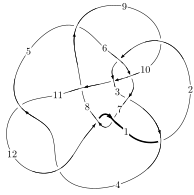
\includegraphics[width=112pt]{../../../GIT/diagram.site/Diagrams/png/1688_12a_0887.png}\\
\ \ \ A knot diagram\footnotemark}&
\allowdisplaybreaks
\textbf{Linearized knot diagam} \\
\cline{2-2}
 &
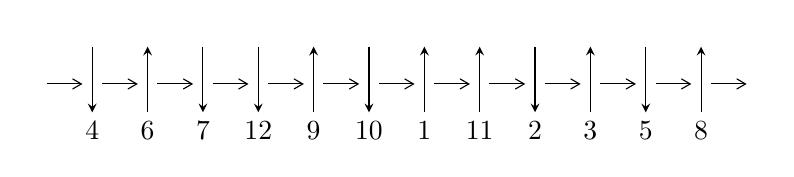
\begin{tikzpicture}[x=20pt, y=17pt]
	% nodes
	\node (C0) at (0, 0) {};
	\node (C1) at (1, 0) {};
	\node (C1U) at (1, +1) {};
	\node (C1D) at (1, -1) {4};

	\node (C2) at (2, 0) {};
	\node (C2U) at (2, +1) {};
	\node (C2D) at (2, -1) {6};

	\node (C3) at (3, 0) {};
	\node (C3U) at (3, +1) {};
	\node (C3D) at (3, -1) {7};

	\node (C4) at (4, 0) {};
	\node (C4U) at (4, +1) {};
	\node (C4D) at (4, -1) {12};

	\node (C5) at (5, 0) {};
	\node (C5U) at (5, +1) {};
	\node (C5D) at (5, -1) {9};

	\node (C6) at (6, 0) {};
	\node (C6U) at (6, +1) {};
	\node (C6D) at (6, -1) {10};

	\node (C7) at (7, 0) {};
	\node (C7U) at (7, +1) {};
	\node (C7D) at (7, -1) {1};

	\node (C8) at (8, 0) {};
	\node (C8U) at (8, +1) {};
	\node (C8D) at (8, -1) {11};

	\node (C9) at (9, 0) {};
	\node (C9U) at (9, +1) {};
	\node (C9D) at (9, -1) {2};

	\node (C10) at (10, 0) {};
	\node (C10U) at (10, +1) {};
	\node (C10D) at (10, -1) {3};

	\node (C11) at (11, 0) {};
	\node (C11U) at (11, +1) {};
	\node (C11D) at (11, -1) {5};

	\node (C12) at (12, 0) {};
	\node (C12U) at (12, +1) {};
	\node (C12D) at (12, -1) {8};
	\node (C13) at (13, 0) {};

	% arrows
	\draw[->,>={angle 60}]
	(C0) edge (C1) (C1) edge (C2) (C2) edge (C3) (C3) edge (C4) (C4) edge (C5) (C5) edge (C6) (C6) edge (C7) (C7) edge (C8) (C8) edge (C9) (C9) edge (C10) (C10) edge (C11) (C11) edge (C12) (C12) edge (C13) ;	\draw[->,>=stealth]
	(C1U) edge (C1D) (C2D) edge (C2U) (C3U) edge (C3D) (C4U) edge (C4D) (C5D) edge (C5U) (C6U) edge (C6D) (C7D) edge (C7U) (C8D) edge (C8U) (C9U) edge (C9D) (C10D) edge (C10U) (C11U) edge (C11D) (C12D) edge (C12U) ;
	\end{tikzpicture} \\
\hhline{~~} \\& 
\textbf{Solving Sequence} \\ \cline{2-2} 
 &
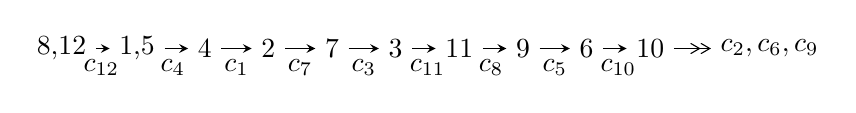
\begin{tikzpicture}[x=23pt, y=7pt]
	% node
	\node (A0) at (-1/8, 0) {8,12};
	\node (A1) at (17/16, 0) {1,5};
	\node (A2) at (17/8, 0) {4};
	\node (A3) at (25/8, 0) {2};
	\node (A4) at (33/8, 0) {7};
	\node (A5) at (41/8, 0) {3};
	\node (A6) at (49/8, 0) {11};
	\node (A7) at (57/8, 0) {9};
	\node (A8) at (65/8, 0) {6};
	\node (A9) at (73/8, 0) {10};
	\node (C1) at (1/2, -1) {$c_{12}$};
	\node (C2) at (13/8, -1) {$c_{4}$};
	\node (C3) at (21/8, -1) {$c_{1}$};
	\node (C4) at (29/8, -1) {$c_{7}$};
	\node (C5) at (37/8, -1) {$c_{3}$};
	\node (C6) at (45/8, -1) {$c_{11}$};
	\node (C7) at (53/8, -1) {$c_{8}$};
	\node (C8) at (61/8, -1) {$c_{5}$};
	\node (C9) at (69/8, -1) {$c_{10}$};
	\node (A10) at (11, 0) {$c_{2},c_{6},c_{9}$};

	% edge
	\draw[->,>=stealth]	
	(A0) edge (A1) (A1) edge (A2) (A2) edge (A3) (A3) edge (A4) (A4) edge (A5) (A5) edge (A6) (A6) edge (A7) (A7) edge (A8) (A8) edge (A9) ;
	\draw[->>,>={angle 60}]	
	(A9) edge (A10);
\end{tikzpicture} \\ 

\end{tabular} \\

\footnotetext{
The image of knot diagram is generated by the software ``\textbf{Draw programme}" developed by Andrew Bartholomew(\url{http://www.layer8.co.uk/maths/draw/index.htm\#Running-draw}), where we modified some parts for our purpose(\url{https://github.com/CATsTAILs/LinksPainter}).
}\phantom \\ \newline 
\centering \textbf{Ideals for irreducible components\footnotemark of $X_{\text{par}}$} 
 
\begin{align*}
I^u_{1}&=\langle 
-7.22780\times10^{1306} u^{189}+2.45986\times10^{1306} u^{188}+\cdots+1.66697\times10^{1306} b-2.31380\times10^{1310},\\
\phantom{I^u_{1}}&\phantom{= \langle  }6.30404\times10^{1315} u^{189}+1.68808\times10^{1315} u^{188}+\cdots+5.96446\times10^{1314} a-5.48078\times10^{1319},\\
\phantom{I^u_{1}}&\phantom{= \langle  }u^{190}+67 u^{188}+\cdots-138006 u-17447\rangle \\
I^u_{2}&=\langle 
9.76518\times10^{48} u^{45}+1.28953\times10^{49} u^{44}+\cdots+7.60878\times10^{48} b-1.58720\times10^{49},\\
\phantom{I^u_{2}}&\phantom{= \langle  }4.78561\times10^{49} u^{45}+3.77004\times10^{49} u^{44}+\cdots+1.52176\times10^{49} a-4.81006\times10^{49},\;u^{46}+u^{45}+\cdots-2 u+1\rangle \\
\\
\end{align*}
\raggedright * 2 irreducible components of $\dim_{\mathbb{C}}=0$, with total 236 representations.\\
\footnotetext{All coefficients of polynomials are rational numbers. But the coefficients are sometimes approximated in decimal forms when there is not enough margin.}
\newpage
\renewcommand{\arraystretch}{1}
\centering \section*{I. $I^u_{1}= \langle -7.23\times10^{1306} u^{189}+2.46\times10^{1306} u^{188}+\cdots+1.67\times10^{1306} b-2.31\times10^{1310},\;6.30\times10^{1315} u^{189}+1.69\times10^{1315} u^{188}+\cdots+5.96\times10^{1314} a-5.48\times10^{1319},\;u^{190}+67 u^{188}+\cdots-138006 u-17447 \rangle$}
\flushleft \textbf{(i) Arc colorings}\\
\begin{tabular}{m{7pt} m{180pt} m{7pt} m{180pt} }
\flushright $a_{8}=$&$\begin{pmatrix}0\\u\end{pmatrix}$ \\
\flushright $a_{12}=$&$\begin{pmatrix}1\\0\end{pmatrix}$ \\
\flushright $a_{1}=$&$\begin{pmatrix}1\\- u^2\end{pmatrix}$ \\
\flushright $a_{5}=$&$\begin{pmatrix}-10.5693 u^{189}-2.83023 u^{188}+\cdots+945060. u+91890.7\\4.33589 u^{189}-1.47565 u^{188}+\cdots+15990.1 u+13880.3\end{pmatrix}$ \\
\flushright $a_{4}=$&$\begin{pmatrix}-6.23344 u^{189}-4.30588 u^{188}+\cdots+961050. u+105771.\\4.33589 u^{189}-1.47565 u^{188}+\cdots+15990.1 u+13880.3\end{pmatrix}$ \\
\flushright $a_{2}=$&$\begin{pmatrix}10.7355 u^{189}+14.2863 u^{188}+\cdots-2.78517\times10^{6} u-323181.\\-4.61634 u^{189}-0.542985 u^{188}+\cdots+199375. u+10795.3\end{pmatrix}$ \\
\flushright $a_{7}=$&$\begin{pmatrix}- u\\u^3+u\end{pmatrix}$ \\
\flushright $a_{3}=$&$\begin{pmatrix}-8.78606 u^{189}-1.37271 u^{188}+\cdots+631875. u+56427.2\\5.22398 u^{189}-1.52033 u^{188}+\cdots-15094.2 u+12049.1\end{pmatrix}$ \\
\flushright $a_{11}=$&$\begin{pmatrix}-5.04397 u^{189}-0.399550 u^{188}+\cdots+172980. u+5773.97\\1.95804 u^{189}-1.48337 u^{188}+\cdots+114320. u+22056.1\end{pmatrix}$ \\
\flushright $a_{9}=$&$\begin{pmatrix}23.6821 u^{189}-2.17840 u^{188}+\cdots-309586. u+26789.7\\-2.09425 u^{189}+0.305661 u^{188}+\cdots-172398. u-26443.0\end{pmatrix}$ \\
\flushright $a_{6}=$&$\begin{pmatrix}15.2253 u^{189}+0.780421 u^{188}+\cdots-624926. u-33479.8\\-0.887353 u^{189}+6.08852 u^{188}+\cdots-1.08620\times10^{6} u-143525.\end{pmatrix}$ \\
\flushright $a_{10}=$&$\begin{pmatrix}-5.78169 u^{189}-5.37501 u^{188}+\cdots+1.18082\times10^{6} u+131470.\\4.03607 u^{189}-1.68248 u^{188}+\cdots+92118.3 u+24863.1\end{pmatrix}$\\&\end{tabular}
\flushleft \textbf{(ii) Obstruction class $= -1$}\\~\\
\flushleft \textbf{(iii) Cusp Shapes $= -4.73829 u^{189}-0.820069 u^{188}+\cdots+142554. u+11834.1$}\\~\\
\newpage\renewcommand{\arraystretch}{1}
\flushleft \textbf{(iv) u-Polynomials at the component}\newline \\
\begin{tabular}{m{50pt}|m{274pt}}
Crossings & \hspace{64pt}u-Polynomials at each crossing \\
\hline $$\begin{aligned}c_{1}\end{aligned}$$&$\begin{aligned}
&u^{190}+5 u^{189}+\cdots+6665 u+199
\end{aligned}$\\
\hline $$\begin{aligned}c_{2}\end{aligned}$$&$\begin{aligned}
&u^{190}-9 u^{189}+\cdots-4 u+1
\end{aligned}$\\
\hline $$\begin{aligned}c_{3}\end{aligned}$$&$\begin{aligned}
&u^{190}-2 u^{189}+\cdots+670900166 u-53862673
\end{aligned}$\\
\hline $$\begin{aligned}c_{4},c_{11}\end{aligned}$$&$\begin{aligned}
&u^{190}+67 u^{188}+\cdots+138006 u-17447
\end{aligned}$\\
\hline $$\begin{aligned}c_{5}\end{aligned}$$&$\begin{aligned}
&u^{190}+2 u^{189}+\cdots-670900166 u-53862673
\end{aligned}$\\
\hline $$\begin{aligned}c_{6}\end{aligned}$$&$\begin{aligned}
&u^{190}+9 u^{189}+\cdots+4 u+1
\end{aligned}$\\
\hline $$\begin{aligned}c_{7},c_{12}\end{aligned}$$&$\begin{aligned}
&u^{190}+67 u^{188}+\cdots-138006 u-17447
\end{aligned}$\\
\hline $$\begin{aligned}c_{8}\end{aligned}$$&$\begin{aligned}
&u^{190}-5 u^{189}+\cdots-6665 u+199
\end{aligned}$\\
\hline $$\begin{aligned}c_{9}\end{aligned}$$&$\begin{aligned}
&u^{190}- u^{189}+\cdots+29 u-1
\end{aligned}$\\
\hline $$\begin{aligned}c_{10}\end{aligned}$$&$\begin{aligned}
&u^{190}+u^{189}+\cdots-29 u-1
\end{aligned}$\\
\hline
\end{tabular}\\~\\
\newpage\renewcommand{\arraystretch}{1}
\flushleft \textbf{(v) Riley Polynomials at the component}\newline \\
\begin{tabular}{m{50pt}|m{274pt}}
Crossings & \hspace{64pt}Riley Polynomials at each crossing \\
\hline $$\begin{aligned}c_{1},c_{8}\end{aligned}$$&$\begin{aligned}
&y^{190}-19 y^{189}+\cdots+1497025 y+39601
\end{aligned}$\\
\hline $$\begin{aligned}c_{2},c_{6}\end{aligned}$$&$\begin{aligned}
&y^{190}-23 y^{189}+\cdots-252 y+1
\end{aligned}$\\
\hline $$\begin{aligned}c_{3},c_{5}\end{aligned}$$&$\begin{aligned}
&y^{190}-88 y^{189}+\cdots-175498183281035406 y+2901187542704929
\end{aligned}$\\
\hline $$\begin{aligned}c_{4},c_{7},c_{11}\\c_{12}\end{aligned}$$&$\begin{aligned}
&y^{190}+134 y^{189}+\cdots+46421594 y+304397809
\end{aligned}$\\
\hline $$\begin{aligned}c_{9},c_{10}\end{aligned}$$&$\begin{aligned}
&y^{190}+23 y^{189}+\cdots-149 y+1
\end{aligned}$\\
\hline
\end{tabular}\\~\\
\newpage\flushleft \textbf{(vi) Complex Volumes and Cusp Shapes}
$$\begin{array}{c|c|c}  
\text{Solutions to }I^u_{1}& \I (\text{vol} + \sqrt{-1}CS) & \text{Cusp shape}\\
 \hline 
\begin{aligned}
u &= -0.864219 + 0.506539 I \\
a &= \phantom{-}0.21689 + 2.29034 I \\
b &= -0.186777 - 1.246840 I\end{aligned}
 & \phantom{-}3.78459 - 4.20222 I & \phantom{-0.000000 } 0 \\ \hline\begin{aligned}
u &= -0.864219 - 0.506539 I \\
a &= \phantom{-}0.21689 - 2.29034 I \\
b &= -0.186777 + 1.246840 I\end{aligned}
 & \phantom{-}3.78459 + 4.20222 I & \phantom{-0.000000 } 0 \\ \hline\begin{aligned}
u &= -0.638373 + 0.767389 I \\
a &= \phantom{-}0.60552 - 2.35236 I \\
b &= \phantom{-}0.080709 + 1.272450 I\end{aligned}
 & \phantom{-}5.21796 - 2.67365 I & \phantom{-0.000000 } 0 \\ \hline\begin{aligned}
u &= -0.638373 - 0.767389 I \\
a &= \phantom{-}0.60552 + 2.35236 I \\
b &= \phantom{-}0.080709 - 1.272450 I\end{aligned}
 & \phantom{-}5.21796 + 2.67365 I & \phantom{-0.000000 } 0 \\ \hline\begin{aligned}
u &= \phantom{-}0.031691 + 0.990579 I \\
a &= -1.37887 + 0.60361 I \\
b &= -0.698418 - 1.148540 I\end{aligned}
 & -1.80089 - 1.83392 I & \phantom{-0.000000 } 0 \\ \hline\begin{aligned}
u &= \phantom{-}0.031691 - 0.990579 I \\
a &= -1.37887 - 0.60361 I \\
b &= -0.698418 + 1.148540 I\end{aligned}
 & -1.80089 + 1.83392 I & \phantom{-0.000000 } 0 \\ \hline\begin{aligned}
u &= -0.340233 + 0.924142 I \\
a &= -1.17546 + 1.01173 I \\
b &= -0.84402 - 1.34401 I\end{aligned}
 & \phantom{-}2.65028 - 5.98733 I & \phantom{-0.000000 } 0 \\ \hline\begin{aligned}
u &= -0.340233 - 0.924142 I \\
a &= -1.17546 - 1.01173 I \\
b &= -0.84402 + 1.34401 I\end{aligned}
 & \phantom{-}2.65028 + 5.98733 I & \phantom{-0.000000 } 0 \\ \hline\begin{aligned}
u &= -0.098449 + 0.972581 I \\
a &= -0.58409 + 1.58122 I \\
b &= -0.16055 - 1.59671 I\end{aligned}
 & \phantom{-}2.01485 - 3.55741 I & \phantom{-0.000000 } 0 \\ \hline\begin{aligned}
u &= -0.098449 - 0.972581 I \\
a &= -0.58409 - 1.58122 I \\
b &= -0.16055 + 1.59671 I\end{aligned}
 & \phantom{-}2.01485 + 3.55741 I & \phantom{-0.000000 } 0\\
 \hline 
 \end{array}$$\newpage$$\begin{array}{c|c|c}  
\text{Solutions to }I^u_{1}& \I (\text{vol} + \sqrt{-1}CS) & \text{Cusp shape}\\
 \hline 
\begin{aligned}
u &= \phantom{-}0.119296 + 0.965852 I \\
a &= \phantom{-}0.017329 - 0.417748 I \\
b &= \phantom{-}0.71740 + 2.20998 I\end{aligned}
 & \phantom{-}0.94548 + 7.07618 I & \phantom{-0.000000 } 0 \\ \hline\begin{aligned}
u &= \phantom{-}0.119296 - 0.965852 I \\
a &= \phantom{-}0.017329 + 0.417748 I \\
b &= \phantom{-}0.71740 - 2.20998 I\end{aligned}
 & \phantom{-}0.94548 - 7.07618 I & \phantom{-0.000000 } 0 \\ \hline\begin{aligned}
u &= \phantom{-}0.613232 + 0.823675 I \\
a &= \phantom{-}0.599902 + 1.103490 I \\
b &= \phantom{-}0.354486 - 1.137680 I\end{aligned}
 & \phantom{-}0.64534 + 2.48885 I & \phantom{-0.000000 } 0 \\ \hline\begin{aligned}
u &= \phantom{-}0.613232 - 0.823675 I \\
a &= \phantom{-}0.599902 - 1.103490 I \\
b &= \phantom{-}0.354486 + 1.137680 I\end{aligned}
 & \phantom{-}0.64534 - 2.48885 I & \phantom{-0.000000 } 0 \\ \hline\begin{aligned}
u &= \phantom{-}0.565862 + 0.787510 I \\
a &= \phantom{-}0.838198 + 0.988520 I \\
b &= \phantom{-}0.612638 - 1.195610 I\end{aligned}
 & \phantom{-}0.82965 + 2.65878 I & \phantom{-0.000000 } 0 \\ \hline\begin{aligned}
u &= \phantom{-}0.565862 - 0.787510 I \\
a &= \phantom{-}0.838198 - 0.988520 I \\
b &= \phantom{-}0.612638 + 1.195610 I\end{aligned}
 & \phantom{-}0.82965 - 2.65878 I & \phantom{-0.000000 } 0 \\ \hline\begin{aligned}
u &= -0.102463 + 0.962021 I \\
a &= -1.50913 - 0.91650 I \\
b &= -0.282652 + 0.856538 I\end{aligned}
 & -3.02895 - 2.54150 I & \phantom{-0.000000 } 0 \\ \hline\begin{aligned}
u &= -0.102463 - 0.962021 I \\
a &= -1.50913 + 0.91650 I \\
b &= -0.282652 - 0.856538 I\end{aligned}
 & -3.02895 + 2.54150 I & \phantom{-0.000000 } 0 \\ \hline\begin{aligned}
u &= \phantom{-}0.048183 + 1.034830 I \\
a &= \phantom{-}0.128851 + 0.373299 I \\
b &= \phantom{-}0.826802 - 0.254280 I\end{aligned}
 & -1.68569 + 1.98753 I & \phantom{-0.000000 } 0 \\ \hline\begin{aligned}
u &= \phantom{-}0.048183 - 1.034830 I \\
a &= \phantom{-}0.128851 - 0.373299 I \\
b &= \phantom{-}0.826802 + 0.254280 I\end{aligned}
 & -1.68569 - 1.98753 I & \phantom{-0.000000 } 0\\
 \hline 
 \end{array}$$\newpage$$\begin{array}{c|c|c}  
\text{Solutions to }I^u_{1}& \I (\text{vol} + \sqrt{-1}CS) & \text{Cusp shape}\\
 \hline 
\begin{aligned}
u &= -0.143691 + 0.946403 I \\
a &= -0.858770 + 0.173939 I \\
b &= -0.96058 - 1.31302 I\end{aligned}
 & \phantom{-}2.04273 - 1.92425 I & \phantom{-0.000000 } 0 \\ \hline\begin{aligned}
u &= -0.143691 - 0.946403 I \\
a &= -0.858770 - 0.173939 I \\
b &= -0.96058 + 1.31302 I\end{aligned}
 & \phantom{-}2.04273 + 1.92425 I & \phantom{-0.000000 } 0 \\ \hline\begin{aligned}
u &= -0.552887 + 0.776994 I \\
a &= -1.21485 + 1.44966 I \\
b &= -0.552887 - 0.776994 I\end{aligned}
 & \phantom{-0.000000 } -5.13061 I & \phantom{-0.000000 } 0 \\ \hline\begin{aligned}
u &= -0.552887 - 0.776994 I \\
a &= -1.21485 - 1.44966 I \\
b &= -0.552887 + 0.776994 I\end{aligned}
 & \phantom{-0.000000 -}5.13061 I & \phantom{-0.000000 } 0 \\ \hline\begin{aligned}
u &= \phantom{-}0.671960 + 0.807813 I \\
a &= \phantom{-}0.339432 + 0.012190 I \\
b &= -0.189179 - 0.240700 I\end{aligned}
 & \phantom{-}0.60621 + 2.56467 I & \phantom{-0.000000 } 0 \\ \hline\begin{aligned}
u &= \phantom{-}0.671960 - 0.807813 I \\
a &= \phantom{-}0.339432 - 0.012190 I \\
b &= -0.189179 + 0.240700 I\end{aligned}
 & \phantom{-}0.60621 - 2.56467 I & \phantom{-0.000000 } 0 \\ \hline\begin{aligned}
u &= -0.155008 + 1.051230 I \\
a &= \phantom{-}0.50273 - 1.94901 I \\
b &= \phantom{-}0.204387 + 1.100630 I\end{aligned}
 & -2.86286 - 4.82970 I & \phantom{-0.000000 } 0 \\ \hline\begin{aligned}
u &= -0.155008 - 1.051230 I \\
a &= \phantom{-}0.50273 + 1.94901 I \\
b &= \phantom{-}0.204387 - 1.100630 I\end{aligned}
 & -2.86286 + 4.82970 I & \phantom{-0.000000 } 0 \\ \hline\begin{aligned}
u &= \phantom{-}0.906525 + 0.226741 I \\
a &= \phantom{-}0.28195 + 1.46628 I \\
b &= -0.252765 - 1.375860 I\end{aligned}
 & \phantom{-}7.99660 + 1.83983 I & \phantom{-0.000000 } 0 \\ \hline\begin{aligned}
u &= \phantom{-}0.906525 - 0.226741 I \\
a &= \phantom{-}0.28195 - 1.46628 I \\
b &= -0.252765 + 1.375860 I\end{aligned}
 & \phantom{-}7.99660 - 1.83983 I & \phantom{-0.000000 } 0\\
 \hline 
 \end{array}$$\newpage$$\begin{array}{c|c|c}  
\text{Solutions to }I^u_{1}& \I (\text{vol} + \sqrt{-1}CS) & \text{Cusp shape}\\
 \hline 
\begin{aligned}
u &= \phantom{-}0.384605 + 1.005630 I \\
a &= \phantom{-}0.530220 + 0.793332 I \\
b &= \phantom{-}0.838496 - 0.137029 I\end{aligned}
 & -0.91300 + 3.25049 I & \phantom{-0.000000 } 0 \\ \hline\begin{aligned}
u &= \phantom{-}0.384605 - 1.005630 I \\
a &= \phantom{-}0.530220 - 0.793332 I \\
b &= \phantom{-}0.838496 + 0.137029 I\end{aligned}
 & -0.91300 - 3.25049 I & \phantom{-0.000000 } 0 \\ \hline\begin{aligned}
u &= \phantom{-}0.081765 + 1.085650 I \\
a &= \phantom{-}2.30031 + 1.57765 I \\
b &= \phantom{-}0.358880 - 1.125930 I\end{aligned}
 & -1.03850 + 9.71041 I & \phantom{-0.000000 } 0 \\ \hline\begin{aligned}
u &= \phantom{-}0.081765 - 1.085650 I \\
a &= \phantom{-}2.30031 - 1.57765 I \\
b &= \phantom{-}0.358880 + 1.125930 I\end{aligned}
 & -1.03850 - 9.71041 I & \phantom{-0.000000 } 0 \\ \hline\begin{aligned}
u &= \phantom{-}0.994147 + 0.447540 I \\
a &= -0.477464 - 1.163730 I \\
b &= \phantom{-}0.390802 + 1.300370 I\end{aligned}
 & \phantom{-}6.58758 - 7.24408 I & \phantom{-0.000000 } 0 \\ \hline\begin{aligned}
u &= \phantom{-}0.994147 - 0.447540 I \\
a &= -0.477464 + 1.163730 I \\
b &= \phantom{-}0.390802 - 1.300370 I\end{aligned}
 & \phantom{-}6.58758 + 7.24408 I & \phantom{-0.000000 } 0 \\ \hline\begin{aligned}
u &= -0.282652 + 0.856538 I \\
a &= \phantom{-}1.89217 - 0.34272 I \\
b &= -0.102463 + 0.962021 I\end{aligned}
 & \phantom{-}3.02895 + 2.54150 I & \phantom{-0.000000 } 0 \\ \hline\begin{aligned}
u &= -0.282652 - 0.856538 I \\
a &= \phantom{-}1.89217 + 0.34272 I \\
b &= -0.102463 - 0.962021 I\end{aligned}
 & \phantom{-}3.02895 - 2.54150 I & \phantom{-0.000000 } 0 \\ \hline\begin{aligned}
u &= -0.013025 + 0.889984 I \\
a &= \phantom{-}0.58377 - 2.54777 I \\
b &= \phantom{-}0.165168 + 1.387130 I\end{aligned}
 & \phantom{-}4.14677 - 4.21274 I & \phantom{-0.000000 } 0 \\ \hline\begin{aligned}
u &= -0.013025 - 0.889984 I \\
a &= \phantom{-}0.58377 + 2.54777 I \\
b &= \phantom{-}0.165168 - 1.387130 I\end{aligned}
 & \phantom{-}4.14677 + 4.21274 I & \phantom{-0.000000 } 0\\
 \hline 
 \end{array}$$\newpage$$\begin{array}{c|c|c}  
\text{Solutions to }I^u_{1}& \I (\text{vol} + \sqrt{-1}CS) & \text{Cusp shape}\\
 \hline 
\begin{aligned}
u &= -1.028930 + 0.419517 I \\
a &= \phantom{-}0.71297 - 1.37414 I \\
b &= -0.178544 + 1.263810 I\end{aligned}
 & \phantom{-}5.05665 + 1.27721 I & \phantom{-0.000000 } 0 \\ \hline\begin{aligned}
u &= -1.028930 - 0.419517 I \\
a &= \phantom{-}0.71297 + 1.37414 I \\
b &= -0.178544 - 1.263810 I\end{aligned}
 & \phantom{-}5.05665 - 1.27721 I & \phantom{-0.000000 } 0 \\ \hline\begin{aligned}
u &= -0.835416 + 0.282230 I \\
a &= -0.09605 - 1.80726 I \\
b &= \phantom{-}0.342270 + 1.368570 I\end{aligned}
 & \phantom{-}4.52184 - 6.28312 I & \phantom{-0.000000 } 0 \\ \hline\begin{aligned}
u &= -0.835416 - 0.282230 I \\
a &= -0.09605 + 1.80726 I \\
b &= \phantom{-}0.342270 - 1.368570 I\end{aligned}
 & \phantom{-}4.52184 + 6.28312 I & \phantom{-0.000000 } 0 \\ \hline\begin{aligned}
u &= \phantom{-}0.204387 + 1.100630 I \\
a &= -0.895943 + 0.544333 I \\
b &= -0.155008 + 1.051230 I\end{aligned}
 & \phantom{-}2.86286 + 4.82970 I & \phantom{-0.000000 } 0 \\ \hline\begin{aligned}
u &= \phantom{-}0.204387 - 1.100630 I \\
a &= -0.895943 - 0.544333 I \\
b &= -0.155008 - 1.051230 I\end{aligned}
 & \phantom{-}2.86286 - 4.82970 I & \phantom{-0.000000 } 0 \\ \hline\begin{aligned}
u &= \phantom{-}0.724429 + 0.492186 I \\
a &= -0.221354 - 0.003732 I \\
b &= \phantom{-}0.218270 - 0.363227 I\end{aligned}
 & \phantom{-}1.06409 + 2.53770 I & \phantom{-0.000000 } 0 \\ \hline\begin{aligned}
u &= \phantom{-}0.724429 - 0.492186 I \\
a &= -0.221354 + 0.003732 I \\
b &= \phantom{-}0.218270 + 0.363227 I\end{aligned}
 & \phantom{-}1.06409 - 2.53770 I & \phantom{-0.000000 } 0 \\ \hline\begin{aligned}
u &= \phantom{-}0.098846 + 1.120500 I \\
a &= -1.32602 - 0.75884 I \\
b &= -0.547775 + 1.014710 I\end{aligned}
 & -4.40175 + 2.27220 I & \phantom{-0.000000 } 0 \\ \hline\begin{aligned}
u &= \phantom{-}0.098846 - 1.120500 I \\
a &= -1.32602 + 0.75884 I \\
b &= -0.547775 - 1.014710 I\end{aligned}
 & -4.40175 - 2.27220 I & \phantom{-0.000000 } 0\\
 \hline 
 \end{array}$$\newpage$$\begin{array}{c|c|c}  
\text{Solutions to }I^u_{1}& \I (\text{vol} + \sqrt{-1}CS) & \text{Cusp shape}\\
 \hline 
\begin{aligned}
u &= -0.038169 + 0.872769 I \\
a &= \phantom{-}3.19060 + 0.29768 I \\
b &= -0.038169 - 0.872769 I\end{aligned}
 & \phantom{-0.000000 } -9.40180 I & \phantom{-0.000000 } 0 \\ \hline\begin{aligned}
u &= -0.038169 - 0.872769 I \\
a &= \phantom{-}3.19060 - 0.29768 I \\
b &= -0.038169 + 0.872769 I\end{aligned}
 & \phantom{-0.000000 -}9.40180 I & \phantom{-0.000000 } 0 \\ \hline\begin{aligned}
u &= \phantom{-}0.826802 + 0.254280 I \\
a &= \phantom{-}0.423229 + 1.072870 I \\
b &= \phantom{-}0.048183 - 1.034830 I\end{aligned}
 & \phantom{-}1.68569 + 1.98753 I & \phantom{-0.000000 } 0 \\ \hline\begin{aligned}
u &= \phantom{-}0.826802 - 0.254280 I \\
a &= \phantom{-}0.423229 - 1.072870 I \\
b &= \phantom{-}0.048183 + 1.034830 I\end{aligned}
 & \phantom{-}1.68569 - 1.98753 I & \phantom{-0.000000 } 0 \\ \hline\begin{aligned}
u &= -0.025027 + 1.137880 I \\
a &= -0.93249 + 1.12429 I \\
b &= -0.135474 - 0.844110 I\end{aligned}
 & -2.26284 + 2.38006 I & \phantom{-0.000000 } 0 \\ \hline\begin{aligned}
u &= -0.025027 - 1.137880 I \\
a &= -0.93249 - 1.12429 I \\
b &= -0.135474 + 0.844110 I\end{aligned}
 & -2.26284 - 2.38006 I & \phantom{-0.000000 } 0 \\ \hline\begin{aligned}
u &= -0.135474 + 0.844110 I \\
a &= -1.46572 - 0.11078 I \\
b &= -0.025027 - 1.137880 I\end{aligned}
 & \phantom{-}2.26284 + 2.38006 I & \phantom{-0.000000 } 0 \\ \hline\begin{aligned}
u &= -0.135474 - 0.844110 I \\
a &= -1.46572 + 0.11078 I \\
b &= -0.025027 + 1.137880 I\end{aligned}
 & \phantom{-}2.26284 - 2.38006 I & \phantom{-0.000000 } 0 \\ \hline\begin{aligned}
u &= -0.073562 + 0.849661 I \\
a &= -0.129598 + 0.600967 I \\
b &= \phantom{-}0.33723 - 1.80064 I\end{aligned}
 & \phantom{-}2.52076 + 0.62563 I & \phantom{-0.000000 } 0 \\ \hline\begin{aligned}
u &= -0.073562 - 0.849661 I \\
a &= -0.129598 - 0.600967 I \\
b &= \phantom{-}0.33723 + 1.80064 I\end{aligned}
 & \phantom{-}2.52076 - 0.62563 I & \phantom{-0.000000 } 0\\
 \hline 
 \end{array}$$\newpage$$\begin{array}{c|c|c}  
\text{Solutions to }I^u_{1}& \I (\text{vol} + \sqrt{-1}CS) & \text{Cusp shape}\\
 \hline 
\begin{aligned}
u &= \phantom{-}0.838496 + 0.137029 I \\
a &= \phantom{-}0.46437 + 1.86669 I \\
b &= \phantom{-}0.384605 - 1.005630 I\end{aligned}
 & \phantom{-}0.91300 + 3.25049 I & \phantom{-0.000000 } 0 \\ \hline\begin{aligned}
u &= \phantom{-}0.838496 - 0.137029 I \\
a &= \phantom{-}0.46437 - 1.86669 I \\
b &= \phantom{-}0.384605 + 1.005630 I\end{aligned}
 & \phantom{-}0.91300 - 3.25049 I & \phantom{-0.000000 } 0 \\ \hline\begin{aligned}
u &= \phantom{-}1.047380 + 0.476835 I \\
a &= \phantom{-}0.44512 + 1.34264 I \\
b &= -0.201455 - 0.670663 I\end{aligned}
 & -1.58375 + 3.04276 I & \phantom{-0.000000 } 0 \\ \hline\begin{aligned}
u &= \phantom{-}1.047380 - 0.476835 I \\
a &= \phantom{-}0.44512 - 1.34264 I \\
b &= -0.201455 + 0.670663 I\end{aligned}
 & -1.58375 - 3.04276 I & \phantom{-0.000000 } 0 \\ \hline\begin{aligned}
u &= -0.547775 + 1.014710 I \\
a &= \phantom{-}1.38852 - 1.21465 I \\
b &= \phantom{-}0.098846 + 1.120500 I\end{aligned}
 & \phantom{-}4.40175 - 2.27220 I & \phantom{-0.000000 } 0 \\ \hline\begin{aligned}
u &= -0.547775 - 1.014710 I \\
a &= \phantom{-}1.38852 + 1.21465 I \\
b &= \phantom{-}0.098846 - 1.120500 I\end{aligned}
 & \phantom{-}4.40175 + 2.27220 I & \phantom{-0.000000 } 0 \\ \hline\begin{aligned}
u &= -0.504260 + 1.039200 I \\
a &= \phantom{-}0.85543 - 1.43473 I \\
b &= \phantom{-}0.45680 + 1.37653 I\end{aligned}
 & \phantom{-}3.25392 - 6.73569 I & \phantom{-0.000000 } 0 \\ \hline\begin{aligned}
u &= -0.504260 - 1.039200 I \\
a &= \phantom{-}0.85543 + 1.43473 I \\
b &= \phantom{-}0.45680 - 1.37653 I\end{aligned}
 & \phantom{-}3.25392 + 6.73569 I & \phantom{-0.000000 } 0 \\ \hline\begin{aligned}
u &= -0.801920 + 0.225074 I \\
a &= \phantom{-}0.26580 - 1.92824 I \\
b &= -0.347240 + 1.306480 I\end{aligned}
 & \phantom{-}6.09129 + 3.67687 I & \phantom{-0.000000 } 0 \\ \hline\begin{aligned}
u &= -0.801920 - 0.225074 I \\
a &= \phantom{-}0.26580 + 1.92824 I \\
b &= -0.347240 - 1.306480 I\end{aligned}
 & \phantom{-}6.09129 - 3.67687 I & \phantom{-0.000000 } 0\\
 \hline 
 \end{array}$$\newpage$$\begin{array}{c|c|c}  
\text{Solutions to }I^u_{1}& \I (\text{vol} + \sqrt{-1}CS) & \text{Cusp shape}\\
 \hline 
\begin{aligned}
u &= -0.194135 + 1.159610 I \\
a &= \phantom{-}0.426812 - 0.802608 I \\
b &= \phantom{-}0.64980 + 1.77633 I\end{aligned}
 & -1.24450 - 6.61929 I & \phantom{-0.000000 } 0 \\ \hline\begin{aligned}
u &= -0.194135 - 1.159610 I \\
a &= \phantom{-}0.426812 + 0.802608 I \\
b &= \phantom{-}0.64980 - 1.77633 I\end{aligned}
 & -1.24450 + 6.61929 I & \phantom{-0.000000 } 0 \\ \hline\begin{aligned}
u &= -0.413869 + 0.712030 I \\
a &= -0.924236 + 0.596977 I \\
b &= \phantom{-}0.40116 - 1.43664 I\end{aligned}
 & \phantom{-}3.26014 + 2.74200 I & \phantom{-0.000000 } 0 \\ \hline\begin{aligned}
u &= -0.413869 - 0.712030 I \\
a &= -0.924236 - 0.596977 I \\
b &= \phantom{-}0.40116 + 1.43664 I\end{aligned}
 & \phantom{-}3.26014 - 2.74200 I & \phantom{-0.000000 } 0 \\ \hline\begin{aligned}
u &= \phantom{-}0.358880 + 1.125930 I \\
a &= \phantom{-}2.42751 + 0.53129 I \\
b &= \phantom{-}0.081765 - 1.085650 I\end{aligned}
 & \phantom{-}1.03850 + 9.71041 I & \phantom{-0.000000 } 0 \\ \hline\begin{aligned}
u &= \phantom{-}0.358880 - 1.125930 I \\
a &= \phantom{-}2.42751 - 0.53129 I \\
b &= \phantom{-}0.081765 + 1.085650 I\end{aligned}
 & \phantom{-}1.03850 - 9.71041 I & \phantom{-0.000000 } 0 \\ \hline\begin{aligned}
u &= \phantom{-}0.354486 + 1.137680 I \\
a &= \phantom{-}0.459887 + 0.682483 I \\
b &= \phantom{-}0.613232 - 0.823675 I\end{aligned}
 & -0.64534 + 2.48885 I & \phantom{-0.000000 } 0 \\ \hline\begin{aligned}
u &= \phantom{-}0.354486 - 1.137680 I \\
a &= \phantom{-}0.459887 - 0.682483 I \\
b &= \phantom{-}0.613232 + 0.823675 I\end{aligned}
 & -0.64534 - 2.48885 I & \phantom{-0.000000 } 0 \\ \hline\begin{aligned}
u &= \phantom{-}0.729973 + 0.296590 I \\
a &= \phantom{-}0.844925 + 0.526610 I \\
b &= -0.542269 - 0.003712 I\end{aligned}
 & \phantom{-}1.50001 + 2.85730 I & \phantom{-0.000000 } 0 \\ \hline\begin{aligned}
u &= \phantom{-}0.729973 - 0.296590 I \\
a &= \phantom{-}0.844925 - 0.526610 I \\
b &= -0.542269 + 0.003712 I\end{aligned}
 & \phantom{-}1.50001 - 2.85730 I & \phantom{-0.000000 } 0\\
 \hline 
 \end{array}$$\newpage$$\begin{array}{c|c|c}  
\text{Solutions to }I^u_{1}& \I (\text{vol} + \sqrt{-1}CS) & \text{Cusp shape}\\
 \hline 
\begin{aligned}
u &= -1.217430 + 0.146682 I \\
a &= \phantom{-}0.35174 - 1.59271 I \\
b &= -0.380162 + 1.230360 I\end{aligned}
 & \phantom{-}5.13554 + 6.54586 I & \phantom{-0.000000 } 0 \\ \hline\begin{aligned}
u &= -1.217430 - 0.146682 I \\
a &= \phantom{-}0.35174 + 1.59271 I \\
b &= -0.380162 - 1.230360 I\end{aligned}
 & \phantom{-}5.13554 - 6.54586 I & \phantom{-0.000000 } 0 \\ \hline\begin{aligned}
u &= \phantom{-}0.640629 + 0.432937 I \\
a &= \phantom{-}0.753849 + 0.653524 I \\
b &= -0.202385 - 1.215850 I\end{aligned}
 & \phantom{-}1.70567 + 1.64873 I & \phantom{-0.000000 } 0 \\ \hline\begin{aligned}
u &= \phantom{-}0.640629 - 0.432937 I \\
a &= \phantom{-}0.753849 - 0.653524 I \\
b &= -0.202385 + 1.215850 I\end{aligned}
 & \phantom{-}1.70567 - 1.64873 I & \phantom{-0.000000 } 0 \\ \hline\begin{aligned}
u &= -0.202385 + 1.215850 I \\
a &= -0.017736 + 0.493749 I \\
b &= \phantom{-}0.640629 - 0.432937 I\end{aligned}
 & -1.70567 + 1.64873 I & \phantom{-0.000000 } 0 \\ \hline\begin{aligned}
u &= -0.202385 - 1.215850 I \\
a &= -0.017736 - 0.493749 I \\
b &= \phantom{-}0.640629 + 0.432937 I\end{aligned}
 & -1.70567 - 1.64873 I & \phantom{-0.000000 } 0 \\ \hline\begin{aligned}
u &= \phantom{-}1.241660 + 0.000578 I \\
a &= -0.103343 - 1.406140 I \\
b &= \phantom{-}0.348304 + 1.259150 I\end{aligned}
 & \phantom{-}2.99999 - 6.53096 I & \phantom{-0.000000 } 0 \\ \hline\begin{aligned}
u &= \phantom{-}1.241660 - 0.000578 I \\
a &= -0.103343 + 1.406140 I \\
b &= \phantom{-}0.348304 - 1.259150 I\end{aligned}
 & \phantom{-}2.99999 + 6.53096 I & \phantom{-0.000000 } 0 \\ \hline\begin{aligned}
u &= -0.735451 + 0.177578 I \\
a &= \phantom{-}0.553053 - 0.678758 I \\
b &= -0.735451 - 0.177578 I\end{aligned}
 & \phantom{-0.000000 } -10.8593 I & \phantom{-0.000000 } 0 \\ \hline\begin{aligned}
u &= -0.735451 - 0.177578 I \\
a &= \phantom{-}0.553053 + 0.678758 I \\
b &= -0.735451 + 0.177578 I\end{aligned}
 & \phantom{-0.000000 -}10.8593 I & \phantom{-0.000000 } 0\\
 \hline 
 \end{array}$$\newpage$$\begin{array}{c|c|c}  
\text{Solutions to }I^u_{1}& \I (\text{vol} + \sqrt{-1}CS) & \text{Cusp shape}\\
 \hline 
\begin{aligned}
u &= \phantom{-}0.592458 + 1.097850 I \\
a &= -0.89786 - 1.10652 I \\
b &= -0.69048 + 1.34634 I\end{aligned}
 & \phantom{-}4.48445 + 12.89690 I & \phantom{-0.000000 } 0 \\ \hline\begin{aligned}
u &= \phantom{-}0.592458 - 1.097850 I \\
a &= -0.89786 + 1.10652 I \\
b &= -0.69048 - 1.34634 I\end{aligned}
 & \phantom{-}4.48445 - 12.89690 I & \phantom{-0.000000 } 0 \\ \hline\begin{aligned}
u &= -1.008240 + 0.736346 I \\
a &= \phantom{-}0.125074 - 0.933280 I \\
b &= -0.141427 + 0.502698 I\end{aligned}
 & -1.61642 + 5.68271 I & \phantom{-0.000000 } 0 \\ \hline\begin{aligned}
u &= -1.008240 - 0.736346 I \\
a &= \phantom{-}0.125074 + 0.933280 I \\
b &= -0.141427 - 0.502698 I\end{aligned}
 & -1.61642 - 5.68271 I & \phantom{-0.000000 } 0 \\ \hline\begin{aligned}
u &= -0.186777 + 1.246840 I \\
a &= -0.760603 - 0.330859 I \\
b &= -0.864219 - 0.506539 I\end{aligned}
 & -3.78459 - 4.20222 I & \phantom{-0.000000 } 0 \\ \hline\begin{aligned}
u &= -0.186777 - 1.246840 I \\
a &= -0.760603 + 0.330859 I \\
b &= -0.864219 + 0.506539 I\end{aligned}
 & -3.78459 + 4.20222 I & \phantom{-0.000000 } 0 \\ \hline\begin{aligned}
u &= \phantom{-}1.274010 + 0.002155 I \\
a &= \phantom{-}0.17769 + 1.53470 I \\
b &= -0.392076 - 1.290980 I\end{aligned}
 & \phantom{-}4.3631 - 14.9744 I & \phantom{-0.000000 } 0 \\ \hline\begin{aligned}
u &= \phantom{-}1.274010 - 0.002155 I \\
a &= \phantom{-}0.17769 - 1.53470 I \\
b &= -0.392076 + 1.290980 I\end{aligned}
 & \phantom{-}4.3631 + 14.9744 I & \phantom{-0.000000 } 0 \\ \hline\begin{aligned}
u &= \phantom{-}0.080709 + 1.272450 I \\
a &= -0.971199 + 0.245399 I \\
b &= -0.638373 + 0.767389 I\end{aligned}
 & -5.21796 + 2.67365 I & \phantom{-0.000000 } 0 \\ \hline\begin{aligned}
u &= \phantom{-}0.080709 - 1.272450 I \\
a &= -0.971199 - 0.245399 I \\
b &= -0.638373 - 0.767389 I\end{aligned}
 & -5.21796 - 2.67365 I & \phantom{-0.000000 } 0\\
 \hline 
 \end{array}$$\newpage$$\begin{array}{c|c|c}  
\text{Solutions to }I^u_{1}& \I (\text{vol} + \sqrt{-1}CS) & \text{Cusp shape}\\
 \hline 
\begin{aligned}
u &= -0.178544 + 1.263810 I \\
a &= -0.317193 - 0.353665 I \\
b &= -1.028930 + 0.419517 I\end{aligned}
 & -5.05665 - 1.27721 I & \phantom{-0.000000 } 0 \\ \hline\begin{aligned}
u &= -0.178544 - 1.263810 I \\
a &= -0.317193 + 0.353665 I \\
b &= -1.028930 - 0.419517 I\end{aligned}
 & -5.05665 + 1.27721 I & \phantom{-0.000000 } 0 \\ \hline\begin{aligned}
u &= -0.435716 + 1.204860 I \\
a &= \phantom{-}1.34640 - 1.04943 I \\
b &= \phantom{-}0.510008 + 1.287380 I\end{aligned}
 & \phantom{-}3.01615 - 8.22973 I & \phantom{-0.000000 } 0 \\ \hline\begin{aligned}
u &= -0.435716 - 1.204860 I \\
a &= \phantom{-}1.34640 + 1.04943 I \\
b &= \phantom{-}0.510008 - 1.287380 I\end{aligned}
 & \phantom{-}3.01615 + 8.22973 I & \phantom{-0.000000 } 0 \\ \hline\begin{aligned}
u &= -0.380162 + 1.230360 I \\
a &= -0.304080 + 0.165278 I \\
b &= -1.217430 + 0.146682 I\end{aligned}
 & -5.13554 - 6.54586 I & \phantom{-0.000000 } 0 \\ \hline\begin{aligned}
u &= -0.380162 - 1.230360 I \\
a &= -0.304080 - 0.165278 I \\
b &= -1.217430 - 0.146682 I\end{aligned}
 & -5.13554 + 6.54586 I & \phantom{-0.000000 } 0 \\ \hline\begin{aligned}
u &= \phantom{-}0.209467 + 1.275540 I \\
a &= -0.310130 - 0.170895 I \\
b &= -1.365010 + 0.227003 I\end{aligned}
 & -5.80644 + 4.40592 I & \phantom{-0.000000 } 0 \\ \hline\begin{aligned}
u &= \phantom{-}0.209467 - 1.275540 I \\
a &= -0.310130 + 0.170895 I \\
b &= -1.365010 - 0.227003 I\end{aligned}
 & -5.80644 - 4.40592 I & \phantom{-0.000000 } 0 \\ \hline\begin{aligned}
u &= -0.008032 + 0.707209 I \\
a &= -0.744637 + 0.267026 I \\
b &= -1.21653 + 0.96709 I\end{aligned}
 & \phantom{-}1.61685 - 5.65859 I & \phantom{-0.000000 } 0 \\ \hline\begin{aligned}
u &= -0.008032 - 0.707209 I \\
a &= -0.744637 - 0.267026 I \\
b &= -1.21653 - 0.96709 I\end{aligned}
 & \phantom{-}1.61685 + 5.65859 I & \phantom{-0.000000 } 0\\
 \hline 
 \end{array}$$\newpage$$\begin{array}{c|c|c}  
\text{Solutions to }I^u_{1}& \I (\text{vol} + \sqrt{-1}CS) & \text{Cusp shape}\\
 \hline 
\begin{aligned}
u &= \phantom{-}0.521757 + 1.190380 I \\
a &= \phantom{-}0.982881 + 0.877814 I \\
b &= \phantom{-}0.57949 - 1.33670 I\end{aligned}
 & \phantom{-}5.01183 + 3.30390 I & \phantom{-0.000000 } 0 \\ \hline\begin{aligned}
u &= \phantom{-}0.521757 - 1.190380 I \\
a &= \phantom{-}0.982881 - 0.877814 I \\
b &= \phantom{-}0.57949 + 1.33670 I\end{aligned}
 & \phantom{-}5.01183 - 3.30390 I & \phantom{-0.000000 } 0 \\ \hline\begin{aligned}
u &= -0.201455 + 0.670663 I \\
a &= \phantom{-}1.094690 - 0.426052 I \\
b &= \phantom{-}1.047380 - 0.476835 I\end{aligned}
 & \phantom{-}1.58375 + 3.04276 I & \phantom{-0.000000 } 0 \\ \hline\begin{aligned}
u &= -0.201455 - 0.670663 I \\
a &= \phantom{-}1.094690 + 0.426052 I \\
b &= \phantom{-}1.047380 + 0.476835 I\end{aligned}
 & \phantom{-}1.58375 - 3.04276 I & \phantom{-0.000000 } 0 \\ \hline\begin{aligned}
u &= \phantom{-}0.348304 + 1.259150 I \\
a &= \phantom{-}0.072451 + 0.261668 I \\
b &= \phantom{-}1.241660 + 0.000578 I\end{aligned}
 & -2.99999 + 6.53096 I & \phantom{-0.000000 } 0 \\ \hline\begin{aligned}
u &= \phantom{-}0.348304 - 1.259150 I \\
a &= \phantom{-}0.072451 - 0.261668 I \\
b &= \phantom{-}1.241660 - 0.000578 I\end{aligned}
 & -2.99999 - 6.53096 I & \phantom{-0.000000 } 0 \\ \hline\begin{aligned}
u &= -0.015741 + 1.325840 I \\
a &= \phantom{-}0.440036 - 0.885792 I \\
b &= \phantom{-}0.498678 - 0.330608 I\end{aligned}
 & -3.42745 - 6.17744 I & \phantom{-0.000000 } 0 \\ \hline\begin{aligned}
u &= -0.015741 - 1.325840 I \\
a &= \phantom{-}0.440036 + 0.885792 I \\
b &= \phantom{-}0.498678 + 0.330608 I\end{aligned}
 & -3.42745 + 6.17744 I & \phantom{-0.000000 } 0 \\ \hline\begin{aligned}
u &= \phantom{-}0.612638 + 1.195610 I \\
a &= \phantom{-}0.345226 + 0.999956 I \\
b &= \phantom{-}0.565862 - 0.787510 I\end{aligned}
 & -0.82965 + 2.65878 I & \phantom{-0.000000 } 0 \\ \hline\begin{aligned}
u &= \phantom{-}0.612638 - 1.195610 I \\
a &= \phantom{-}0.345226 - 0.999956 I \\
b &= \phantom{-}0.565862 + 0.787510 I\end{aligned}
 & -0.82965 - 2.65878 I & \phantom{-0.000000 } 0\\
 \hline 
 \end{array}$$\newpage$$\begin{array}{c|c|c}  
\text{Solutions to }I^u_{1}& \I (\text{vol} + \sqrt{-1}CS) & \text{Cusp shape}\\
 \hline 
\begin{aligned}
u &= -0.698418 + 1.148540 I \\
a &= -1.13573 + 1.10329 I \\
b &= \phantom{-}0.031691 - 0.990579 I\end{aligned}
 & \phantom{-}1.80089 - 1.83392 I & \phantom{-0.000000 } 0 \\ \hline\begin{aligned}
u &= -0.698418 - 1.148540 I \\
a &= -1.13573 - 1.10329 I \\
b &= \phantom{-}0.031691 + 0.990579 I\end{aligned}
 & \phantom{-}1.80089 + 1.83392 I & \phantom{-0.000000 } 0 \\ \hline\begin{aligned}
u &= \phantom{-}0.651859\phantom{ +0.000000I} \\
a &= \phantom{-}1.30127\phantom{ +0.000000I} \\
b &= -0.121386\phantom{ +0.000000I}\end{aligned}
 & \phantom{-}1.03935\phantom{ +0.000000I} & \phantom{-0.000000 } 0 \\ \hline\begin{aligned}
u &= -0.392076 + 1.290980 I \\
a &= \phantom{-}0.160934 - 0.260850 I \\
b &= \phantom{-}1.274010 - 0.002155 I\end{aligned}
 & -4.3631 - 14.9744 I & \phantom{-0.000000 } 0 \\ \hline\begin{aligned}
u &= -0.392076 - 1.290980 I \\
a &= \phantom{-}0.160934 + 0.260850 I \\
b &= \phantom{-}1.274010 + 0.002155 I\end{aligned}
 & -4.3631 + 14.9744 I & \phantom{-0.000000 } 0 \\ \hline\begin{aligned}
u &= -0.347240 + 1.306480 I \\
a &= -0.304351 + 0.237992 I \\
b &= -0.801920 + 0.225074 I\end{aligned}
 & -6.09129 - 3.67687 I & \phantom{-0.000000 } 0 \\ \hline\begin{aligned}
u &= -0.347240 - 1.306480 I \\
a &= -0.304351 - 0.237992 I \\
b &= -0.801920 - 0.225074 I\end{aligned}
 & -6.09129 + 3.67687 I & \phantom{-0.000000 } 0 \\ \hline\begin{aligned}
u &= \phantom{-}0.390802 + 1.300370 I \\
a &= -0.0372292 - 0.1244690 I \\
b &= \phantom{-}0.994147 + 0.447540 I\end{aligned}
 & -6.58758 + 7.24408 I & \phantom{-0.000000 } 0 \\ \hline\begin{aligned}
u &= \phantom{-}0.390802 - 1.300370 I \\
a &= -0.0372292 + 0.1244690 I \\
b &= \phantom{-}0.994147 - 0.447540 I\end{aligned}
 & -6.58758 - 7.24408 I & \phantom{-0.000000 } 0 \\ \hline\begin{aligned}
u &= -0.602683 + 0.154149 I \\
a &= \phantom{-}0.339281 + 0.335040 I \\
b &= \phantom{-}0.512946 - 0.069863 I\end{aligned}
 & -1.64259 + 0.07288 I & \phantom{-0.000000 } 0\\
 \hline 
 \end{array}$$\newpage$$\begin{array}{c|c|c}  
\text{Solutions to }I^u_{1}& \I (\text{vol} + \sqrt{-1}CS) & \text{Cusp shape}\\
 \hline 
\begin{aligned}
u &= -0.602683 - 0.154149 I \\
a &= \phantom{-}0.339281 - 0.335040 I \\
b &= \phantom{-}0.512946 + 0.069863 I\end{aligned}
 & -1.64259 - 0.07288 I & \phantom{-0.000000 } 0 \\ \hline\begin{aligned}
u &= -1.365010 + 0.227003 I \\
a &= -0.04924 - 1.56492 I \\
b &= \phantom{-}0.209467 + 1.275540 I\end{aligned}
 & \phantom{-}5.80644 - 4.40592 I & \phantom{-0.000000 } 0 \\ \hline\begin{aligned}
u &= -1.365010 - 0.227003 I \\
a &= -0.04924 + 1.56492 I \\
b &= \phantom{-}0.209467 - 1.275540 I\end{aligned}
 & \phantom{-}5.80644 + 4.40592 I & \phantom{-0.000000 } 0 \\ \hline\begin{aligned}
u &= \phantom{-}0.510008 + 1.287380 I \\
a &= -1.14072 - 1.30291 I \\
b &= -0.435716 + 1.204860 I\end{aligned}
 & -3.01615 + 8.22973 I & \phantom{-0.000000 } 0 \\ \hline\begin{aligned}
u &= \phantom{-}0.510008 - 1.287380 I \\
a &= -1.14072 + 1.30291 I \\
b &= -0.435716 - 1.204860 I\end{aligned}
 & -3.01615 - 8.22973 I & \phantom{-0.000000 } 0 \\ \hline\begin{aligned}
u &= \phantom{-}0.165168 + 1.387130 I \\
a &= -0.571152 + 0.669630 I \\
b &= -0.013025 + 0.889984 I\end{aligned}
 & -4.14677 + 4.21274 I & \phantom{-0.000000 } 0 \\ \hline\begin{aligned}
u &= \phantom{-}0.165168 - 1.387130 I \\
a &= -0.571152 - 0.669630 I \\
b &= -0.013025 - 0.889984 I\end{aligned}
 & -4.14677 - 4.21274 I & \phantom{-0.000000 } 0 \\ \hline\begin{aligned}
u &= -0.252765 + 1.375860 I \\
a &= \phantom{-}0.0630504 - 0.0072569 I \\
b &= \phantom{-}0.906525 - 0.226741 I\end{aligned}
 & -7.99660 + 1.83983 I & \phantom{-0.000000 } 0 \\ \hline\begin{aligned}
u &= -0.252765 - 1.375860 I \\
a &= \phantom{-}0.0630504 + 0.0072569 I \\
b &= \phantom{-}0.906525 + 0.226741 I\end{aligned}
 & -7.99660 - 1.83983 I & \phantom{-0.000000 } 0 \\ \hline\begin{aligned}
u &= \phantom{-}0.498678 + 0.330608 I \\
a &= -1.05892 + 3.23620 I \\
b &= -0.015741 - 1.325840 I\end{aligned}
 & \phantom{-}3.42745 - 6.17744 I & \phantom{-0.000000 } 0\\
 \hline 
 \end{array}$$\newpage$$\begin{array}{c|c|c}  
\text{Solutions to }I^u_{1}& \I (\text{vol} + \sqrt{-1}CS) & \text{Cusp shape}\\
 \hline 
\begin{aligned}
u &= \phantom{-}0.498678 - 0.330608 I \\
a &= -1.05892 - 3.23620 I \\
b &= -0.015741 + 1.325840 I\end{aligned}
 & \phantom{-}3.42745 + 6.17744 I & \phantom{-0.000000 } 0 \\ \hline\begin{aligned}
u &= \phantom{-}0.342270 + 1.368570 I \\
a &= -0.285730 - 0.131290 I \\
b &= -0.835416 + 0.282230 I\end{aligned}
 & -4.52184 + 6.28312 I & \phantom{-0.000000 } 0 \\ \hline\begin{aligned}
u &= \phantom{-}0.342270 - 1.368570 I \\
a &= -0.285730 + 0.131290 I \\
b &= -0.835416 - 0.282230 I\end{aligned}
 & -4.52184 - 6.28312 I & \phantom{-0.000000 } 0 \\ \hline\begin{aligned}
u &= \phantom{-}0.044599 + 0.559522 I \\
a &= \phantom{-}2.19902 + 1.72214 I \\
b &= \phantom{-}0.037178 + 0.336355 I\end{aligned}
 & -1.26339 + 3.53599 I & \phantom{-0.000000 } 0 \\ \hline\begin{aligned}
u &= \phantom{-}0.044599 - 0.559522 I \\
a &= \phantom{-}2.19902 - 1.72214 I \\
b &= \phantom{-}0.037178 - 0.336355 I\end{aligned}
 & -1.26339 - 3.53599 I & \phantom{-0.000000 } 0 \\ \hline\begin{aligned}
u &= \phantom{-}0.45680 + 1.37653 I \\
a &= -0.781031 - 0.695952 I \\
b &= -0.504260 + 1.039200 I\end{aligned}
 & -3.25392 + 6.73569 I & \phantom{-0.000000 } 0 \\ \hline\begin{aligned}
u &= \phantom{-}0.45680 - 1.37653 I \\
a &= -0.781031 + 0.695952 I \\
b &= -0.504260 - 1.039200 I\end{aligned}
 & -3.25392 - 6.73569 I & \phantom{-0.000000 } 0 \\ \hline\begin{aligned}
u &= \phantom{-}0.57949 + 1.33670 I \\
a &= \phantom{-}0.64875 + 1.29975 I \\
b &= \phantom{-}0.521757 - 1.190380 I\end{aligned}
 & -5.01183 + 3.30390 I & \phantom{-0.000000 } 0 \\ \hline\begin{aligned}
u &= \phantom{-}0.57949 - 1.33670 I \\
a &= \phantom{-}0.64875 - 1.29975 I \\
b &= \phantom{-}0.521757 + 1.190380 I\end{aligned}
 & -5.01183 - 3.30390 I & \phantom{-0.000000 } 0 \\ \hline\begin{aligned}
u &= -0.542269 + 0.003712 I \\
a &= \phantom{-}0.127368 - 0.868560 I \\
b &= \phantom{-}0.729973 - 0.296590 I\end{aligned}
 & -1.50001 + 2.85730 I & -7.03168 - 9.29271 I\\
 \hline 
 \end{array}$$\newpage$$\begin{array}{c|c|c}  
\text{Solutions to }I^u_{1}& \I (\text{vol} + \sqrt{-1}CS) & \text{Cusp shape}\\
 \hline 
\begin{aligned}
u &= -0.542269 - 0.003712 I \\
a &= \phantom{-}0.127368 + 0.868560 I \\
b &= \phantom{-}0.729973 + 0.296590 I\end{aligned}
 & -1.50001 - 2.85730 I & -7.03168 + 9.29271 I \\ \hline\begin{aligned}
u &= -0.60249 + 1.33280 I \\
a &= \phantom{-}0.79980 - 1.29573 I \\
b &= \phantom{-}0.58228 + 1.38962 I\end{aligned}
 & \phantom{-}1.35735 - 12.84530 I & \phantom{-0.000000 } 0 \\ \hline\begin{aligned}
u &= -0.60249 - 1.33280 I \\
a &= \phantom{-}0.79980 + 1.29573 I \\
b &= \phantom{-}0.58228 - 1.38962 I\end{aligned}
 & \phantom{-}1.35735 + 12.84530 I & \phantom{-0.000000 } 0 \\ \hline\begin{aligned}
u &= -0.141427 + 0.502698 I \\
a &= -0.605084 + 0.833743 I \\
b &= -1.008240 + 0.736346 I\end{aligned}
 & \phantom{-}1.61642 - 5.68271 I & \phantom{-}5.78893 + 6.51076 I \\ \hline\begin{aligned}
u &= -0.141427 - 0.502698 I \\
a &= -0.605084 - 0.833743 I \\
b &= -1.008240 - 0.736346 I\end{aligned}
 & \phantom{-}1.61642 + 5.68271 I & \phantom{-}5.78893 - 6.51076 I \\ \hline\begin{aligned}
u &= \phantom{-}0.512946 + 0.069863 I \\
a &= \phantom{-}1.053910 - 0.199001 I \\
b &= -0.602683 - 0.154149 I\end{aligned}
 & \phantom{-}1.64259 + 0.07288 I & \phantom{-}6.72266 + 0. I\phantom{ +0.000000I} \\ \hline\begin{aligned}
u &= \phantom{-}0.512946 - 0.069863 I \\
a &= \phantom{-}1.053910 + 0.199001 I \\
b &= -0.602683 + 0.154149 I\end{aligned}
 & \phantom{-}1.64259 - 0.07288 I & \phantom{-}6.72266 + 0. I\phantom{ +0.000000I} \\ \hline\begin{aligned}
u &= -0.45647 + 1.41731 I \\
a &= -0.759777 + 0.979733 I \\
b &= -0.60812 - 1.45626 I\end{aligned}
 & -0.74114 - 11.16110 I & \phantom{-0.000000 } 0 \\ \hline\begin{aligned}
u &= -0.45647 - 1.41731 I \\
a &= -0.759777 - 0.979733 I \\
b &= -0.60812 + 1.45626 I\end{aligned}
 & -0.74114 + 11.16110 I & \phantom{-0.000000 } 0 \\ \hline\begin{aligned}
u &= \phantom{-}0.40116 + 1.43664 I \\
a &= -0.162936 + 0.521349 I \\
b &= -0.413869 - 0.712030 I\end{aligned}
 & -3.26014 + 2.74200 I & \phantom{-0.000000 } 0\\
 \hline 
 \end{array}$$\newpage$$\begin{array}{c|c|c}  
\text{Solutions to }I^u_{1}& \I (\text{vol} + \sqrt{-1}CS) & \text{Cusp shape}\\
 \hline 
\begin{aligned}
u &= \phantom{-}0.40116 - 1.43664 I \\
a &= -0.162936 - 0.521349 I \\
b &= -0.413869 + 0.712030 I\end{aligned}
 & -3.26014 - 2.74200 I & \phantom{-0.000000 } 0 \\ \hline\begin{aligned}
u &= \phantom{-}0.58228 + 1.38962 I \\
a &= -0.847279 - 1.044300 I \\
b &= -0.60249 + 1.33280 I\end{aligned}
 & -1.35735 + 12.84530 I & \phantom{-0.000000 } 0 \\ \hline\begin{aligned}
u &= \phantom{-}0.58228 - 1.38962 I \\
a &= -0.847279 + 1.044300 I \\
b &= -0.60249 - 1.33280 I\end{aligned}
 & -1.35735 - 12.84530 I & \phantom{-0.000000 } 0 \\ \hline\begin{aligned}
u &= -0.69048 + 1.34634 I \\
a &= \phantom{-}0.578684 - 1.191290 I \\
b &= \phantom{-}0.592458 + 1.097850 I\end{aligned}
 & -4.48445 - 12.89690 I & \phantom{-0.000000 } 0 \\ \hline\begin{aligned}
u &= -0.69048 - 1.34634 I \\
a &= \phantom{-}0.578684 + 1.191290 I \\
b &= \phantom{-}0.592458 - 1.097850 I\end{aligned}
 & -4.48445 + 12.89690 I & \phantom{-0.000000 } 0 \\ \hline\begin{aligned}
u &= \phantom{-}0.59787 + 1.39664 I \\
a &= \phantom{-}0.83451 + 1.18352 I \\
b &= \phantom{-}0.59787 - 1.39664 I\end{aligned}
 & \phantom{-0.000000 -}21.4390 I & \phantom{-0.000000 } 0 \\ \hline\begin{aligned}
u &= \phantom{-}0.59787 - 1.39664 I \\
a &= \phantom{-}0.83451 - 1.18352 I \\
b &= \phantom{-}0.59787 + 1.39664 I\end{aligned}
 & \phantom{-0.000000 } -21.4390 I & \phantom{-0.000000 } 0 \\ \hline\begin{aligned}
u &= -1.21653 + 0.96709 I \\
a &= \phantom{-}0.127649 - 1.046760 I \\
b &= -0.008032 + 0.707209 I\end{aligned}
 & -1.61685 + 5.65859 I & \phantom{-0.000000 } 0 \\ \hline\begin{aligned}
u &= -1.21653 - 0.96709 I \\
a &= \phantom{-}0.127649 + 1.046760 I \\
b &= -0.008032 - 0.707209 I\end{aligned}
 & -1.61685 - 5.65859 I & \phantom{-0.000000 } 0 \\ \hline\begin{aligned}
u &= \phantom{-}0.218270 + 0.363227 I \\
a &= -0.757589 + 0.035843 I \\
b &= \phantom{-}0.724429 - 0.492186 I\end{aligned}
 & -1.06409 + 2.53770 I & -9.83616 - 8.02353 I\\
 \hline 
 \end{array}$$\newpage$$\begin{array}{c|c|c}  
\text{Solutions to }I^u_{1}& \I (\text{vol} + \sqrt{-1}CS) & \text{Cusp shape}\\
 \hline 
\begin{aligned}
u &= \phantom{-}0.218270 - 0.363227 I \\
a &= -0.757589 - 0.035843 I \\
b &= \phantom{-}0.724429 + 0.492186 I\end{aligned}
 & -1.06409 - 2.53770 I & -9.83616 + 8.02353 I \\ \hline\begin{aligned}
u &= -0.60812 + 1.45626 I \\
a &= -0.689061 + 1.180300 I \\
b &= -0.45647 - 1.41731 I\end{aligned}
 & \phantom{-}0.74114 - 11.16110 I & \phantom{-0.000000 } 0 \\ \hline\begin{aligned}
u &= -0.60812 - 1.45626 I \\
a &= -0.689061 - 1.180300 I \\
b &= -0.45647 + 1.41731 I\end{aligned}
 & \phantom{-}0.74114 + 11.16110 I & \phantom{-0.000000 } 0 \\ \hline\begin{aligned}
u &= -0.84402 + 1.34401 I \\
a &= -0.602391 + 1.118000 I \\
b &= -0.340233 - 0.924142 I\end{aligned}
 & -2.65028 - 5.98733 I & \phantom{-0.000000 } 0 \\ \hline\begin{aligned}
u &= -0.84402 - 1.34401 I \\
a &= -0.602391 - 1.118000 I \\
b &= -0.340233 + 0.924142 I\end{aligned}
 & -2.65028 + 5.98733 I & \phantom{-0.000000 } 0 \\ \hline\begin{aligned}
u &= -0.16055 + 1.59671 I \\
a &= -0.442577 + 0.099851 I \\
b &= -0.098449 - 0.972581 I\end{aligned}
 & -2.01485 - 3.55741 I & \phantom{-0.000000 } 0 \\ \hline\begin{aligned}
u &= -0.16055 - 1.59671 I \\
a &= -0.442577 - 0.099851 I \\
b &= -0.098449 + 0.972581 I\end{aligned}
 & -2.01485 + 3.55741 I & \phantom{-0.000000 } 0 \\ \hline\begin{aligned}
u &= -0.96058 + 1.31302 I \\
a &= -0.286862 + 1.230000 I \\
b &= -0.143691 - 0.946403 I\end{aligned}
 & -2.04273 - 1.92425 I & \phantom{-0.000000 } 0 \\ \hline\begin{aligned}
u &= -0.96058 - 1.31302 I \\
a &= -0.286862 - 1.230000 I \\
b &= -0.143691 + 0.946403 I\end{aligned}
 & -2.04273 + 1.92425 I & \phantom{-0.000000 } 0 \\ \hline\begin{aligned}
u &= \phantom{-}0.037178 + 0.336355 I \\
a &= -3.60309 - 3.52603 I \\
b &= \phantom{-}0.044599 + 0.559522 I\end{aligned}
 & \phantom{-}1.26339 - 3.53599 I & \phantom{-}8.48761 + 1.84732 I\\
 \hline 
 \end{array}$$\newpage$$\begin{array}{c|c|c}  
\text{Solutions to }I^u_{1}& \I (\text{vol} + \sqrt{-1}CS) & \text{Cusp shape}\\
 \hline 
\begin{aligned}
u &= \phantom{-}0.037178 - 0.336355 I \\
a &= -3.60309 + 3.52603 I \\
b &= \phantom{-}0.044599 - 0.559522 I\end{aligned}
 & \phantom{-}1.26339 + 3.53599 I & \phantom{-}8.48761 - 1.84732 I \\ \hline\begin{aligned}
u &= -0.189179 + 0.240700 I \\
a &= \phantom{-}0.493757 + 0.798291 I \\
b &= \phantom{-}0.671960 - 0.807813 I\end{aligned}
 & -0.60621 + 2.56467 I & \phantom{-}1.05348 + 9.91926 I \\ \hline\begin{aligned}
u &= -0.189179 - 0.240700 I \\
a &= \phantom{-}0.493757 - 0.798291 I \\
b &= \phantom{-}0.671960 + 0.807813 I\end{aligned}
 & -0.60621 - 2.56467 I & \phantom{-}1.05348 - 9.91926 I \\ \hline\begin{aligned}
u &= \phantom{-}0.33723 + 1.80064 I \\
a &= \phantom{-}0.041114 + 0.565302 I \\
b &= -0.073562 - 0.849661 I\end{aligned}
 & -2.52076 + 0.62563 I & \phantom{-0.000000 } 0 \\ \hline\begin{aligned}
u &= \phantom{-}0.33723 - 1.80064 I \\
a &= \phantom{-}0.041114 - 0.565302 I \\
b &= -0.073562 + 0.849661 I\end{aligned}
 & -2.52076 - 0.62563 I & \phantom{-0.000000 } 0 \\ \hline\begin{aligned}
u &= -0.121386\phantom{ +0.000000I} \\
a &= \phantom{-}6.33618\phantom{ +0.000000I} \\
b &= \phantom{-}0.651859\phantom{ +0.000000I}\end{aligned}
 & -1.03935\phantom{ +0.000000I} & -9.23360\phantom{ +0.000000I} \\ \hline\begin{aligned}
u &= \phantom{-}0.64980 + 1.77633 I \\
a &= -0.282970 - 0.856836 I \\
b &= -0.194135 + 1.159610 I\end{aligned}
 & \phantom{-}1.24450 + 6.61929 I & \phantom{-0.000000 } 0 \\ \hline\begin{aligned}
u &= \phantom{-}0.64980 - 1.77633 I \\
a &= -0.282970 + 0.856836 I \\
b &= -0.194135 - 1.159610 I\end{aligned}
 & \phantom{-}1.24450 - 6.61929 I & \phantom{-0.000000 } 0 \\ \hline\begin{aligned}
u &= \phantom{-}0.71740 + 2.20998 I \\
a &= -0.159639 - 0.795440 I \\
b &= \phantom{-}0.119296 + 0.965852 I\end{aligned}
 & -0.94548 - 7.07618 I & \phantom{-0.000000 } 0 \\ \hline\begin{aligned}
u &= \phantom{-}0.71740 - 2.20998 I \\
a &= -0.159639 + 0.795440 I \\
b &= \phantom{-}0.119296 - 0.965852 I\end{aligned}
 & -0.94548 + 7.07618 I & \phantom{-0.000000 } 0\\
 \hline 
 \end{array}$$\newpage\newpage\renewcommand{\arraystretch}{1}
\centering \section*{II. $I^u_{2}= \langle 9.77\times10^{48} u^{45}+1.29\times10^{49} u^{44}+\cdots+7.61\times10^{48} b-1.59\times10^{49},\;4.79\times10^{49} u^{45}+3.77\times10^{49} u^{44}+\cdots+1.52\times10^{49} a-4.81\times10^{49},\;u^{46}+u^{45}+\cdots-2 u+1 \rangle$}
\flushleft \textbf{(i) Arc colorings}\\
\begin{tabular}{m{7pt} m{180pt} m{7pt} m{180pt} }
\flushright $a_{8}=$&$\begin{pmatrix}0\\u\end{pmatrix}$ \\
\flushright $a_{12}=$&$\begin{pmatrix}1\\0\end{pmatrix}$ \\
\flushright $a_{1}=$&$\begin{pmatrix}1\\- u^2\end{pmatrix}$ \\
\flushright $a_{5}=$&$\begin{pmatrix}-3.14479 u^{45}-2.47743 u^{44}+\cdots+6.20769 u+3.16086\\-1.28341 u^{45}-1.69479 u^{44}+\cdots+6.32515 u+2.08601\end{pmatrix}$ \\
\flushright $a_{4}=$&$\begin{pmatrix}-4.42820 u^{45}-4.17222 u^{44}+\cdots+12.5328 u+5.24687\\-1.28341 u^{45}-1.69479 u^{44}+\cdots+6.32515 u+2.08601\end{pmatrix}$ \\
\flushright $a_{2}=$&$\begin{pmatrix}0.845860 u^{45}+1.58667 u^{44}+\cdots-7.57292 u+13.1916\\-0.942781 u^{45}-1.28190 u^{44}+\cdots+16.0628 u+0.227574\end{pmatrix}$ \\
\flushright $a_{7}=$&$\begin{pmatrix}- u\\u^3+u\end{pmatrix}$ \\
\flushright $a_{3}=$&$\begin{pmatrix}-2.88832 u^{45}-2.72018 u^{44}+\cdots+16.4425 u+5.69110\\-1.88543 u^{45}-2.20767 u^{44}+\cdots+4.13104 u+1.55394\end{pmatrix}$ \\
\flushright $a_{11}=$&$\begin{pmatrix}0.465016 u^{45}-0.995453 u^{44}+\cdots+20.3747 u-8.28756\\1.98562 u^{45}+2.56756 u^{44}+\cdots-11.8551 u-1.10611\end{pmatrix}$ \\
\flushright $a_{9}=$&$\begin{pmatrix}6.47064 u^{45}+3.64790 u^{44}+\cdots+12.8110 u-1.77496\\-2.64343 u^{45}-1.34550 u^{44}+\cdots-12.4888 u-1.73754\end{pmatrix}$ \\
\flushright $a_{6}=$&$\begin{pmatrix}7.15260 u^{45}+5.81205 u^{44}+\cdots-5.90193 u+11.2994\\-2.38129 u^{45}-3.79813 u^{44}+\cdots+14.4459 u-3.26141\end{pmatrix}$ \\
\flushright $a_{10}=$&$\begin{pmatrix}-0.451925 u^{45}-1.49570 u^{44}+\cdots+16.7203 u-12.0040\\0.327833 u^{45}+1.22926 u^{44}+\cdots-17.2272 u+1.86062\end{pmatrix}$\\&\end{tabular}
\flushleft \textbf{(ii) Obstruction class $= 1$}\\~\\
\flushleft \textbf{(iii) Cusp Shapes $= -9.71406 u^{45}-14.4173 u^{44}+\cdots+113.376 u+42.9605$}\\~\\
\newpage\renewcommand{\arraystretch}{1}
\flushleft \textbf{(iv) u-Polynomials at the component}\newline \\
\begin{tabular}{m{50pt}|m{274pt}}
Crossings & \hspace{64pt}u-Polynomials at each crossing \\
\hline $$\begin{aligned}c_{1}\end{aligned}$$&$\begin{aligned}
&u^{46}-10 u^{45}+\cdots-43 u+7
\end{aligned}$\\
\hline $$\begin{aligned}c_{2}\end{aligned}$$&$\begin{aligned}
&u^{46}+4 u^{45}+\cdots-16 u^2+1
\end{aligned}$\\
\hline $$\begin{aligned}c_{3}\end{aligned}$$&$\begin{aligned}
&u^{46}+3 u^{45}+\cdots+6 u+11
\end{aligned}$\\
\hline $$\begin{aligned}c_{4},c_{7}\end{aligned}$$&$\begin{aligned}
&u^{46}- u^{45}+\cdots+2 u+1
\end{aligned}$\\
\hline $$\begin{aligned}c_{5}\end{aligned}$$&$\begin{aligned}
&u^{46}-3 u^{45}+\cdots-6 u+11
\end{aligned}$\\
\hline $$\begin{aligned}c_{6}\end{aligned}$$&$\begin{aligned}
&u^{46}-4 u^{45}+\cdots-16 u^2+1
\end{aligned}$\\
\hline $$\begin{aligned}c_{8}\end{aligned}$$&$\begin{aligned}
&u^{46}+10 u^{45}+\cdots+43 u+7
\end{aligned}$\\
\hline $$\begin{aligned}c_{9}\end{aligned}$$&$\begin{aligned}
&u^{46}+11 u^{44}+\cdots- u+1
\end{aligned}$\\
\hline $$\begin{aligned}c_{10}\end{aligned}$$&$\begin{aligned}
&u^{46}+11 u^{44}+\cdots+u+1
\end{aligned}$\\
\hline $$\begin{aligned}c_{11},c_{12}\end{aligned}$$&$\begin{aligned}
&u^{46}+u^{45}+\cdots-2 u+1
\end{aligned}$\\
\hline
\end{tabular}\\~\\
\newpage\renewcommand{\arraystretch}{1}
\flushleft \textbf{(v) Riley Polynomials at the component}\newline \\
\begin{tabular}{m{50pt}|m{274pt}}
Crossings & \hspace{64pt}Riley Polynomials at each crossing \\
\hline $$\begin{aligned}c_{1},c_{8}\end{aligned}$$&$\begin{aligned}
&y^{46}-4 y^{45}+\cdots-939 y+49
\end{aligned}$\\
\hline $$\begin{aligned}c_{2},c_{6}\end{aligned}$$&$\begin{aligned}
&y^{46}-4 y^{45}+\cdots-32 y+1
\end{aligned}$\\
\hline $$\begin{aligned}c_{3},c_{5}\end{aligned}$$&$\begin{aligned}
&y^{46}-29 y^{45}+\cdots-2522 y+121
\end{aligned}$\\
\hline $$\begin{aligned}c_{4},c_{7},c_{11}\\c_{12}\end{aligned}$$&$\begin{aligned}
&y^{46}+41 y^{45}+\cdots-30 y+1
\end{aligned}$\\
\hline $$\begin{aligned}c_{9},c_{10}\end{aligned}$$&$\begin{aligned}
&y^{46}+22 y^{45}+\cdots+27 y+1
\end{aligned}$\\
\hline
\end{tabular}\\~\\
\newpage\flushleft \textbf{(vi) Complex Volumes and Cusp Shapes}
$$\begin{array}{c|c|c}  
\text{Solutions to }I^u_{2}& \I (\text{vol} + \sqrt{-1}CS) & \text{Cusp shape}\\
 \hline 
\begin{aligned}
u &= \phantom{-}0.727540 + 0.688729 I \\
a &= -0.427620 - 0.261294 I \\
b &= \phantom{-}0.200432 - 0.011361 I\end{aligned}
 & \phantom{-}0.53949 + 2.86039 I & \phantom{-0.000000 } 0. - 15.4305 I \\ \hline\begin{aligned}
u &= \phantom{-}0.727540 - 0.688729 I \\
a &= -0.427620 + 0.261294 I \\
b &= \phantom{-}0.200432 + 0.011361 I\end{aligned}
 & \phantom{-}0.53949 - 2.86039 I & \phantom{-0.000000 -}0. + 15.4305 I \\ \hline\begin{aligned}
u &= -0.329478 + 0.960965 I \\
a &= \phantom{-}1.16986 - 1.12279 I \\
b &= \phantom{-}0.68718 + 1.34568 I\end{aligned}
 & \phantom{-}2.50780 - 5.65241 I & \phantom{-0.000000 } 0 \\ \hline\begin{aligned}
u &= -0.329478 - 0.960965 I \\
a &= \phantom{-}1.16986 + 1.12279 I \\
b &= \phantom{-}0.68718 - 1.34568 I\end{aligned}
 & \phantom{-}2.50780 + 5.65241 I & \phantom{-0.000000 } 0 \\ \hline\begin{aligned}
u &= -0.778009 + 0.584867 I \\
a &= -0.20578 + 2.50673 I \\
b &= -0.105849 - 1.265510 I\end{aligned}
 & \phantom{-}4.47763 - 3.29898 I & \phantom{-}5.18756 + 3.44828 I \\ \hline\begin{aligned}
u &= -0.778009 - 0.584867 I \\
a &= -0.20578 - 2.50673 I \\
b &= -0.105849 + 1.265510 I\end{aligned}
 & \phantom{-}4.47763 + 3.29898 I & \phantom{-}5.18756 - 3.44828 I \\ \hline\begin{aligned}
u &= -1.025180 + 0.087295 I \\
a &= -0.26513 - 1.70468 I \\
b &= \phantom{-}0.327609 + 1.291840 I\end{aligned}
 & \phantom{-}4.78004 - 5.53985 I & \phantom{-0.000000 } 0 \\ \hline\begin{aligned}
u &= -1.025180 - 0.087295 I \\
a &= -0.26513 + 1.70468 I \\
b &= \phantom{-}0.327609 - 1.291840 I\end{aligned}
 & \phantom{-}4.78004 + 5.53985 I & \phantom{-0.000000 } 0 \\ \hline\begin{aligned}
u &= -0.065381 + 0.948354 I \\
a &= \phantom{-}0.660454 + 0.569804 I \\
b &= \phantom{-}0.64687 - 1.77525 I\end{aligned}
 & \phantom{-}0.94522 - 6.65017 I & \phantom{-}1.38744 + 1.69747 I \\ \hline\begin{aligned}
u &= -0.065381 - 0.948354 I \\
a &= \phantom{-}0.660454 - 0.569804 I \\
b &= \phantom{-}0.64687 + 1.77525 I\end{aligned}
 & \phantom{-}0.94522 + 6.65017 I & \phantom{-}1.38744 - 1.69747 I\\
 \hline 
 \end{array}$$\newpage$$\begin{array}{c|c|c}  
\text{Solutions to }I^u_{2}& \I (\text{vol} + \sqrt{-1}CS) & \text{Cusp shape}\\
 \hline 
\begin{aligned}
u &= \phantom{-}0.313371 + 1.008590 I \\
a &= \phantom{-}2.79375 + 1.42100 I \\
b &= \phantom{-}0.313371 - 1.008590 I\end{aligned}
 & \phantom{-0.000000 -}10.6567 I & \phantom{-0.000000 } 0 \\ \hline\begin{aligned}
u &= \phantom{-}0.313371 - 1.008590 I \\
a &= \phantom{-}2.79375 - 1.42100 I \\
b &= \phantom{-}0.313371 + 1.008590 I\end{aligned}
 & \phantom{-0.000000 } -10.6567 I & \phantom{-0.000000 } 0 \\ \hline\begin{aligned}
u &= -0.646822 + 0.591396 I \\
a &= \phantom{-}0.88503 - 1.19039 I \\
b &= \phantom{-}0.586185 + 1.102620 I\end{aligned}
 & \phantom{-}0.54038 - 2.81203 I & -12.74993 + 4.27436 I \\ \hline\begin{aligned}
u &= -0.646822 - 0.591396 I \\
a &= \phantom{-}0.88503 + 1.19039 I \\
b &= \phantom{-}0.586185 - 1.102620 I\end{aligned}
 & \phantom{-}0.54038 + 2.81203 I & -12.74993 - 4.27436 I \\ \hline\begin{aligned}
u &= -0.043894 + 0.833181 I \\
a &= \phantom{-}0.754718 - 0.573028 I \\
b &= \phantom{-}0.55008 + 1.61160 I\end{aligned}
 & \phantom{-}2.62289 - 1.22032 I & \phantom{-}9.80701 + 4.35080 I \\ \hline\begin{aligned}
u &= -0.043894 - 0.833181 I \\
a &= \phantom{-}0.754718 + 0.573028 I \\
b &= \phantom{-}0.55008 - 1.61160 I\end{aligned}
 & \phantom{-}2.62289 + 1.22032 I & \phantom{-}9.80701 - 4.35080 I \\ \hline\begin{aligned}
u &= \phantom{-}0.204267 + 0.736085 I \\
a &= -1.74200 + 0.37937 I \\
b &= -0.442043 + 0.302005 I\end{aligned}
 & \phantom{-}0.80874 + 4.00875 I & \phantom{-}0.23241 - 9.18036 I \\ \hline\begin{aligned}
u &= \phantom{-}0.204267 - 0.736085 I \\
a &= -1.74200 - 0.37937 I \\
b &= -0.442043 - 0.302005 I\end{aligned}
 & \phantom{-}0.80874 - 4.00875 I & \phantom{-}0.23241 + 9.18036 I \\ \hline\begin{aligned}
u &= \phantom{-}0.586185 + 1.102620 I \\
a &= -0.317153 - 0.984578 I \\
b &= -0.646822 + 0.591396 I\end{aligned}
 & -0.54038 + 2.81203 I & \phantom{-0.000000 } 0 \\ \hline\begin{aligned}
u &= \phantom{-}0.586185 - 1.102620 I \\
a &= -0.317153 + 0.984578 I \\
b &= -0.646822 - 0.591396 I\end{aligned}
 & -0.54038 - 2.81203 I & \phantom{-0.000000 } 0\\
 \hline 
 \end{array}$$\newpage$$\begin{array}{c|c|c}  
\text{Solutions to }I^u_{2}& \I (\text{vol} + \sqrt{-1}CS) & \text{Cusp shape}\\
 \hline 
\begin{aligned}
u &= -0.105849 + 1.265510 I \\
a &= -0.932535 - 0.304062 I \\
b &= -0.778009 - 0.584867 I\end{aligned}
 & -4.47763 - 3.29898 I & \phantom{-0.000000 } 0 \\ \hline\begin{aligned}
u &= -0.105849 - 1.265510 I \\
a &= -0.932535 + 0.304062 I \\
b &= -0.778009 + 0.584867 I\end{aligned}
 & -4.47763 + 3.29898 I & \phantom{-0.000000 } 0 \\ \hline\begin{aligned}
u &= -0.320917 + 0.633639 I \\
a &= \phantom{-}1.086150 - 0.393176 I \\
b &= -0.25002 + 1.52526 I\end{aligned}
 & \phantom{-}3.48588 + 2.45562 I & \phantom{-}13.9636 + 3.1362 I \\ \hline\begin{aligned}
u &= -0.320917 - 0.633639 I \\
a &= \phantom{-}1.086150 + 0.393176 I \\
b &= -0.25002 - 1.52526 I\end{aligned}
 & \phantom{-}3.48588 - 2.45562 I & \phantom{-}13.9636 - 3.1362 I \\ \hline\begin{aligned}
u &= \phantom{-}0.136120 + 1.304210 I \\
a &= -0.465825 + 0.953517 I \\
b &= -0.280410 + 0.467502 I\end{aligned}
 & -5.16145 + 4.49240 I & \phantom{-0.000000 } 0 \\ \hline\begin{aligned}
u &= \phantom{-}0.136120 - 1.304210 I \\
a &= -0.465825 - 0.953517 I \\
b &= -0.280410 - 0.467502 I\end{aligned}
 & -5.16145 - 4.49240 I & \phantom{-0.000000 } 0 \\ \hline\begin{aligned}
u &= -0.046914 + 1.325630 I \\
a &= \phantom{-}0.188006 + 0.656992 I \\
b &= -0.046914 - 1.325630 I\end{aligned}
 & \phantom{-0.000000 -}5.87289 I & \phantom{-0.000000 } 0 \\ \hline\begin{aligned}
u &= -0.046914 - 1.325630 I \\
a &= \phantom{-}0.188006 - 0.656992 I \\
b &= -0.046914 + 1.325630 I\end{aligned}
 & \phantom{-0.000000 } -5.87289 I & \phantom{-0.000000 } 0 \\ \hline\begin{aligned}
u &= \phantom{-}0.327609 + 1.291840 I \\
a &= -0.306628 - 0.099445 I \\
b &= -1.025180 + 0.087295 I\end{aligned}
 & -4.78004 + 5.53985 I & \phantom{-0.000000 } 0 \\ \hline\begin{aligned}
u &= \phantom{-}0.327609 - 1.291840 I \\
a &= -0.306628 + 0.099445 I \\
b &= -1.025180 - 0.087295 I\end{aligned}
 & -4.78004 - 5.53985 I & \phantom{-0.000000 } 0\\
 \hline 
 \end{array}$$\newpage$$\begin{array}{c|c|c}  
\text{Solutions to }I^u_{2}& \I (\text{vol} + \sqrt{-1}CS) & \text{Cusp shape}\\
 \hline 
\begin{aligned}
u &= -0.280410 + 0.467502 I \\
a &= -0.61780 - 3.81100 I \\
b &= \phantom{-}0.136120 + 1.304210 I\end{aligned}
 & \phantom{-}5.16145 - 4.49240 I & \phantom{-}10.46065 + 5.83591 I \\ \hline\begin{aligned}
u &= -0.280410 - 0.467502 I \\
a &= -0.61780 + 3.81100 I \\
b &= \phantom{-}0.136120 - 1.304210 I\end{aligned}
 & \phantom{-}5.16145 + 4.49240 I & \phantom{-}10.46065 - 5.83591 I \\ \hline\begin{aligned}
u &= -0.442043 + 0.302005 I \\
a &= \phantom{-}0.08572 - 3.26342 I \\
b &= \phantom{-}0.204267 + 0.736085 I\end{aligned}
 & -0.80874 - 4.00875 I & -0.23241 + 9.18036 I \\ \hline\begin{aligned}
u &= -0.442043 - 0.302005 I \\
a &= \phantom{-}0.08572 + 3.26342 I \\
b &= \phantom{-}0.204267 - 0.736085 I\end{aligned}
 & -0.80874 + 4.00875 I & -0.23241 - 9.18036 I \\ \hline\begin{aligned}
u &= \phantom{-}0.68718 + 1.34568 I \\
a &= -0.759936 - 1.001910 I \\
b &= -0.329478 + 0.960965 I\end{aligned}
 & -2.50780 + 5.65241 I & \phantom{-0.000000 } 0 \\ \hline\begin{aligned}
u &= \phantom{-}0.68718 - 1.34568 I \\
a &= -0.759936 + 1.001910 I \\
b &= -0.329478 - 0.960965 I\end{aligned}
 & -2.50780 - 5.65241 I & \phantom{-0.000000 } 0 \\ \hline\begin{aligned}
u &= -0.54474 + 1.42111 I \\
a &= -0.722129 + 1.091760 I \\
b &= -0.54474 - 1.42111 I\end{aligned}
 & \phantom{-0.000000 } -11.2700 I & \phantom{-0.000000 } 0 \\ \hline\begin{aligned}
u &= -0.54474 - 1.42111 I \\
a &= -0.722129 - 1.091760 I \\
b &= -0.54474 + 1.42111 I\end{aligned}
 & \phantom{-0.000000 -}11.2700 I & \phantom{-0.000000 } 0 \\ \hline\begin{aligned}
u &= -0.25002 + 1.52526 I \\
a &= -0.209460 - 0.611891 I \\
b &= -0.320917 + 0.633639 I\end{aligned}
 & -3.48588 - 2.45562 I & \phantom{-0.000000 } 0 \\ \hline\begin{aligned}
u &= -0.25002 - 1.52526 I \\
a &= -0.209460 + 0.611891 I \\
b &= -0.320917 - 0.633639 I\end{aligned}
 & -3.48588 + 2.45562 I & \phantom{-0.000000 } 0\\
 \hline 
 \end{array}$$\newpage$$\begin{array}{c|c|c}  
\text{Solutions to }I^u_{2}& \I (\text{vol} + \sqrt{-1}CS) & \text{Cusp shape}\\
 \hline 
\begin{aligned}
u &= \phantom{-}0.55008 + 1.61160 I \\
a &= -0.403835 - 0.710308 I \\
b &= -0.043894 + 0.833181 I\end{aligned}
 & -2.62289 + 1.22032 I & \phantom{-0.000000 } 0 \\ \hline\begin{aligned}
u &= \phantom{-}0.55008 - 1.61160 I \\
a &= -0.403835 + 0.710308 I \\
b &= -0.043894 - 0.833181 I\end{aligned}
 & -2.62289 - 1.22032 I & \phantom{-0.000000 } 0 \\ \hline\begin{aligned}
u &= \phantom{-}0.200432 + 0.011361 I \\
a &= -0.21191 - 1.75836 I \\
b &= \phantom{-}0.727540 - 0.688729 I\end{aligned}
 & -0.53949 + 2.86039 I & \phantom{-}6.2042 - 15.4305 I \\ \hline\begin{aligned}
u &= \phantom{-}0.200432 - 0.011361 I \\
a &= -0.21191 + 1.75836 I \\
b &= \phantom{-}0.727540 + 0.688729 I\end{aligned}
 & -0.53949 - 2.86039 I & \phantom{-}6.2042 + 15.4305 I \\ \hline\begin{aligned}
u &= \phantom{-}0.64687 + 1.77525 I \\
a &= \phantom{-}0.464060 + 0.764909 I \\
b &= -0.065381 - 0.948354 I\end{aligned}
 & -0.94522 - 6.65017 I & \phantom{-0.000000 } 0 \\ \hline\begin{aligned}
u &= \phantom{-}0.64687 - 1.77525 I \\
a &= \phantom{-}0.464060 - 0.764909 I \\
b &= -0.065381 + 0.948354 I\end{aligned}
 & -0.94522 + 6.65017 I & \phantom{-0.000000 } 0\\
 \hline 
 \end{array}$$\newpage
\newpage\renewcommand{\arraystretch}{1}
\centering \section*{ III. u-Polynomials}
\begin{tabular}{m{50pt}|m{274pt}}
Crossings & \hspace{64pt}u-Polynomials at each crossing \\
\hline $$\begin{aligned}c_{1}\end{aligned}$$&$\begin{aligned}
&(u^{46}-10 u^{45}+\cdots-43 u+7)(u^{190}+5 u^{189}+\cdots+6665 u+199)
\end{aligned}$\\
\hline $$\begin{aligned}c_{2}\end{aligned}$$&$\begin{aligned}
&(u^{46}+4 u^{45}+\cdots-16 u^2+1)(u^{190}-9 u^{189}+\cdots-4 u+1)
\end{aligned}$\\
\hline $$\begin{aligned}c_{3}\end{aligned}$$&$\begin{aligned}
&(u^{46}+3 u^{45}+\cdots+6 u+11)\\
&\cdot(u^{190}-2 u^{189}+\cdots+670900166 u-53862673)
\end{aligned}$\\
\hline $$\begin{aligned}c_{4}\end{aligned}$$&$\begin{aligned}
&(u^{46}- u^{45}+\cdots+2 u+1)(u^{190}+67 u^{188}+\cdots+138006 u-17447)
\end{aligned}$\\
\hline $$\begin{aligned}c_{5}\end{aligned}$$&$\begin{aligned}
&(u^{46}-3 u^{45}+\cdots-6 u+11)\\
&\cdot(u^{190}+2 u^{189}+\cdots-670900166 u-53862673)
\end{aligned}$\\
\hline $$\begin{aligned}c_{6}\end{aligned}$$&$\begin{aligned}
&(u^{46}-4 u^{45}+\cdots-16 u^2+1)(u^{190}+9 u^{189}+\cdots+4 u+1)
\end{aligned}$\\
\hline $$\begin{aligned}c_{7}\end{aligned}$$&$\begin{aligned}
&(u^{46}- u^{45}+\cdots+2 u+1)(u^{190}+67 u^{188}+\cdots-138006 u-17447)
\end{aligned}$\\
\hline $$\begin{aligned}c_{8}\end{aligned}$$&$\begin{aligned}
&(u^{46}+10 u^{45}+\cdots+43 u+7)(u^{190}-5 u^{189}+\cdots-6665 u+199)
\end{aligned}$\\
\hline $$\begin{aligned}c_{9}\end{aligned}$$&$\begin{aligned}
&(u^{46}+11 u^{44}+\cdots- u+1)(u^{190}- u^{189}+\cdots+29 u-1)
\end{aligned}$\\
\hline $$\begin{aligned}c_{10}\end{aligned}$$&$\begin{aligned}
&(u^{46}+11 u^{44}+\cdots+u+1)(u^{190}+u^{189}+\cdots-29 u-1)
\end{aligned}$\\
\hline $$\begin{aligned}c_{11}\end{aligned}$$&$\begin{aligned}
&(u^{46}+u^{45}+\cdots-2 u+1)(u^{190}+67 u^{188}+\cdots+138006 u-17447)
\end{aligned}$\\
\hline $$\begin{aligned}c_{12}\end{aligned}$$&$\begin{aligned}
&(u^{46}+u^{45}+\cdots-2 u+1)(u^{190}+67 u^{188}+\cdots-138006 u-17447)
\end{aligned}$\\
\hline
\end{tabular}\newpage\renewcommand{\arraystretch}{1}
\centering \section*{ IV. Riley Polynomials}
\begin{tabular}{m{50pt}|m{274pt}}
Crossings & \hspace{64pt}Riley Polynomials at each crossing \\
\hline $$\begin{aligned}c_{1},c_{8}\end{aligned}$$&$\begin{aligned}
&(y^{46}-4 y^{45}+\cdots-939 y+49)\\
&\cdot(y^{190}-19 y^{189}+\cdots+1497025 y+39601)
\end{aligned}$\\
\hline $$\begin{aligned}c_{2},c_{6}\end{aligned}$$&$\begin{aligned}
&(y^{46}-4 y^{45}+\cdots-32 y+1)(y^{190}-23 y^{189}+\cdots-252 y+1)
\end{aligned}$\\
\hline $$\begin{aligned}c_{3},c_{5}\end{aligned}$$&$\begin{aligned}
&(y^{46}-29 y^{45}+\cdots-2522 y+121)\\
&\cdot(y^{190}-88 y^{189}+\cdots-175498183281035406 y+2901187542704929)
\end{aligned}$\\
\hline $$\begin{aligned}c_{4},c_{7},c_{11}\\c_{12}\end{aligned}$$&$\begin{aligned}
&(y^{46}+41 y^{45}+\cdots-30 y+1)\\
&\cdot(y^{190}+134 y^{189}+\cdots+46421594 y+304397809)
\end{aligned}$\\
\hline $$\begin{aligned}c_{9},c_{10}\end{aligned}$$&$\begin{aligned}
&(y^{46}+22 y^{45}+\cdots+27 y+1)(y^{190}+23 y^{189}+\cdots-149 y+1)
\end{aligned}$\\
\hline
\end{tabular}
\vskip 2pc
\end{document}